\section{SLR-Parser}
In this section, we demonstrate how to compute the functions 
\\[0.2cm]
\hspace*{1.3cm}
\(\textsl{action}: Q \times T \rightarrow \textsl{Action}\) \quad and \quad \(\textsl{goto}: Q \times V \rightarrow Q\)
\\[0.2cm]
that have been used in the last section to build a shift-reduce parser for a given context-free grammar \(G\).
For this purpose, we first clarify what information the states contained in the set \(Q\) should hold. We will
define these states in such a way that they contain information about which rule the shift-reduce parser is
attempting to apply, which part of the right hand side of a grammar rule has already been recognized, and what
are the symbols that are still expected. To this end, we define the concept of a \textcolor{blue}{marked rule}.
Unfortunately, the original English literature \cite{knuth:65} uses the rather meaningless term
``\textcolor{blue}{item}'' instead of the notion of a \emph{marked rule}. 

\begin{Definition}[Marked Rule]
  A \textcolor{blue}{marked rule} \index{marked rule} of a context-free grammar \(G = \langle V, T, R, s
  \rangle\) is a triple 
  \\[0.2cm]
  \hspace*{1.3cm}
  \(( a, \beta, \gamma )\),
  \\[0.2cm]
  such that
  \\[0.2cm]
  \hspace*{1.3cm}
  \((a \rightarrow \beta \gamma) \in R\).
  \\[0.2cm]
  A marked rule of the form \(\langle a, \beta, \gamma \rangle\) is written as
  \\[0.2cm]
  \hspace*{1.3cm}
  \(a \rightarrow \beta \bullet \gamma\). \eox
\end{Definition}

\noindent
The marked rule \(a \rightarrow \beta \bullet \gamma\) indicates that the parser is trying to parse an \(a\)
with the rule \(a \rightarrow \beta \gamma\), having already seen \(\beta\) and is next attempting to recognize
\(\gamma\). The symbol \(\bullet\) thus marks the part of the right side of the rule that we have
already read.  Now the idea is to represent a state of an SLR parser as a \blue{set of marked rules}. To illustrate
this idea, let's consider a specific example: we start with the grammar for arithmetic expressions shown in
Figure \ref{fig:Expr.grammar} on page \pageref{fig:Expr.grammar}. We extend this grammar by a new start symbol
\(\widehat{s}\) and the rule 
\\[0.2cm]
\hspace*{1.3cm} \(\widehat{s} \rightarrow  \textsl{expr}\;\symbol{36}\)
\\[0.2cm]
where the symbol ``$\symbol{36}$'' is used to denote \textsc{Eof}, i.e.~the end of the input.
The start state clearly contains the marked rule
\\[0.2cm]
\hspace*{1.3cm} \(\widehat{s} \rightarrow \lambda \bullet \textsl{expr}\; \symbol{36}\),
\\[0.2cm]
since at the beginning we are trying to derive the start symbol \(\widehat{s}\).
The component \(\lambda\) indicates that we have not yet processed anything. In addition to this marked rule, the start state must also contain the marked rules
\begin{enumerate}
\item \(\textsl{expr} \rightarrow \lambda \bullet \textsl{expr} \aquoted{+} \textsl{product}\),
\item \(\textsl{expr} \rightarrow \lambda \bullet \textsl{expr} \aquoted{-} \textsl{product}\) \qquad and
\item \(\textsl{expr} \rightarrow \lambda \bullet \textsl{product}\)
\end{enumerate}
because, for example, it may be necessary to use the rule
\\[0.2cm]
\hspace*{1.3cm}
\(\textsl{expr} \rightarrow \textsl{expr} \aquoted{+} \textsl{product}\)
\\[0.2cm]  
to derive the sought \textsl{expr}. Similarly, it could be that instead we need to use the rule
\\[0.2cm]
\hspace*{1.3cm}
\(\textsl{expr} \rightarrow \textsl{product}\)
\\[0.2cm]
This explains why we must include the marked rule
\\[0.2cm]
\hspace*{1.3cm}
 \(\textsl{expr} \rightarrow \lambda \bullet \textsl{product}\)
\\[0.2cm]
in the start state, because at the beginning we cannot yet know which rule we will need, so the start state must contain all these rules. Once we have added the marked rule
\\[0.2cm]
\hspace*{1.3cm}
 \(\textsl{expr} \rightarrow \lambda \bullet \textsl{product}\) 
\\[0.2cm]
to the start state, we see that we might need to read a \textsl{product} next.  
Therefore, the start state also contains the following marked rules\footnote{In order to be more concise, we
drop the empty string $\lambda$ in the following rules.}:  
\begin{enumerate}
\item[4.] \(\textsl{product} \rightarrow \bullet\; \textsl{product} \aquoted{*} \textsl{factor}\),
\item[5.] \(\textsl{product} \rightarrow \bullet\; \textsl{product} \aquoted{/} \textsl{factor}\),
\item[6.] \(\textsl{product} \rightarrow \bullet\; \textsl{factor}\),

      Now, the sixth rule indicates that we might first read a \textsl{factor}. Therefore, we add the following two marked rules to the start state: 
\item[7.] \(\textsl{factor} \rightarrow \bullet \aquoted{(} \textsl{expr} \aquoted{)}\),
\item[8.] \(\textsl{factor} \rightarrow \bullet\; \textsc{Number}\).
\end{enumerate}
Overall, we see that the start state consists of a set of 8 marked rules.
The system shown above, for deriving further rules from a given rule,
is formalized in the concept of the \textcolor{blue}{closure} of a set of marked rules.

\begin{Definition}[\(\textsl{closure}(\mathcal{M})\)]
  Let \(\mathcal{M}\) be a set of marked rules. Then we define the \textcolor{blue}{closure} \index{closure of a set of marked rules} of this set as the smallest set \(\mathcal{K}\) of marked rules such that:
  \begin{enumerate}
  \item \(\mathcal{M} \subseteq \mathcal{K}\),

        i.e.~the closure includes the original set of rules.
  \item If on the one hand
        \\[0.2cm]
        \hspace*{1.3cm}
        \(a \rightarrow \beta \bullet c\, \delta\)
        \\[0.2cm]
        is a marked rule from the set \(\mathcal{K}\), where \(c\) is a syntactic variable, and on the other hand
        \\[0.2cm]
        \hspace*{1.3cm}
        \(c \rightarrow \gamma\)
        \\[0.2cm]
        is a grammar rule of the underlying grammar \(G\), then the marked rule 
        \\[0.2cm]
        \hspace*{1.3cm}
        \(c \rightarrow \bullet\; \gamma\)
        \\[0.2cm]
        is also an element of the set \(\mathcal{K}\). Formally, this is written as follows:
        \\[0.2cm]
        \hspace*{1.3cm}
        \((a \rightarrow \beta \bullet c\, \delta) \in \mathcal{K} 
         \;\wedge\; 
         (c \rightarrow \gamma) \in R
         \;\Rightarrow\; (c \rightarrow \bullet\; \gamma) \in \mathcal{K}
        \)
  \end{enumerate}
  The set \(\mathcal{K}\) defined in this way is uniquely determined and is referred to as \(\textsl{closure}(\mathcal{M})\) \index{\(\textsl{closure}(\mathcal{M})\)} in the following. \eox
\end{Definition}

\noindent
\textbf{Remark}: If you recall the Earley algorithm, you will notice that the calculation of the closure is the
same as the \emph{prediction operation} in the Earley algorithm. \eox 
\vspace*{0.3cm}

\noindent
For a given set \(\mathcal{M}\) of marked rules, the computation of \(\mathcal{K} := \textsl{closure}(\mathcal{M})\) can be done iteratively:
\begin{enumerate}
\item Initially, set \(\mathcal{K} := \mathcal{M}\).
\item Then, find all rules of the form
      \\[0.2cm]
      \hspace*{1.3cm}
      \(a \rightarrow \beta \bullet c\, \delta\)
      \\[0.2cm]
      within the set \(\mathcal{K}\), where \(c\) is a syntactic variable. Subsequently, for all rules of the form \(c \rightarrow \gamma\), add the new marked rule
      \\[0.2cm]
      \hspace*{1.3cm}
      \(c \rightarrow \bullet\;\gamma\)
      \\[0.2cm]
      into the set \(\mathcal{K}\). Repeat this step until no new rules are found.
\end{enumerate}

\exampleEng
Starting from the grammar for arithmetic expressions shown in Figure \ref{fig:Expr.grammar} on page \pageref{fig:Expr.grammar}, let's consider the set
\[ \mathcal{M} := 
   \bigl\{ \textsl{product} \rightarrow \textsl{product} \aquoted{*}\! \bullet \textsl{factor} \bigr\}
\]
For the set \(\textsl{closure}(\mathcal{M})\), we then find
\\[0.2cm]
\hspace*{1.3cm}
$ 
\begin{array}[b]{lcll}
\textsl{closure}(\mathcal{M}) 
 & = & \bigl\{ &
         \textsl{product} \rightarrow \textsl{product} \aquoted{*}\! \bullet \textsl{factor}, \\
   & & & \textsl{factor}  \rightarrow \bullet \aquoted{(} \textsl{expr} \aquoted{)}\!\!,          \\
   & & & \textsl{factor}  \rightarrow \bullet \;\textsc{Number}                                  \\
   & & \bigr\}. & \hspace*{8cm} 
\end{array}$  \eox
\vspace*{0.3cm}

\noindent
Our goal is to define a Shift-Reduce-Parser
\\[0.2cm]
\hspace*{1.3cm}
\(P = \langle Q, q_0, \textsl{action}, \textsl{goto} \rangle\)
\\[0.2cm]
for a given context-free grammar \(G = \langle V, T, R, s \rangle\). To achieve this goal, we first need to
determine how to define the states in the set \(Q\), as this will almost automatically define the remaining
components. As mentioned earlier, we define the states as sets of marked rules. Let's first define 
\\[0.2cm]
\hspace*{1.3cm}
\(\Gamma := \bigl\{ a \rightarrow \beta \bullet \gamma \mid (a \rightarrow \beta \gamma) \in R \bigr\}\)
\\[0.2cm]
as the set of all marked rules of the grammar. However, it is not sensible to allow arbitrary subsets of
\(\Gamma\) as states: A subset \(\mathcal{M} \subseteq \Gamma\) is only considered as a state if the set
\(\mathcal{M}\) is \blue{closed} under the function \(\textsl{closure}()\), meaning
\(\textsl{closure}(\mathcal{M}) = \mathcal{M}\). Therefore, we define 
\\[0.2cm]
\hspace*{1.3cm}
\(Q := \bigl\{ \mathcal{M} \in 2^\Gamma \mid \textsl{closure}(\mathcal{M}) = \mathcal{M} \bigr\}\).
\\[0.2cm]
The interpretation of the sets \(\mathcal{M} \in Q\) is that a state \(\mathcal{M}\) contains exactly those
marked rules that can be applied in the situation described by the state. 

To simplify the following constructions, we extend the
grammar \(G = \langle V, T, R, s \rangle\) by introducing a new start symbol \(\widehat{s}\)
and a new token \(\symbol{36}\) to the grammar
\\[0.2cm]
\hspace*{1.3cm}
\(\widehat{G} = 
 \Bigl\langle V \cup \{ \widehat{s} \}, T \cup \{\symbol{36}\}, R \cup \{ \widehat{s} \rightarrow s\, \symbol{36} \}, \widehat{s} \Bigr\rangle
\).
\\[0.2cm]
We refer to the grammar \(\widehat{G}\) as the \blue{augmented grammar}.\index{augmented grammar}
The use of the augmented grammar enables the following definition of the start state.
We set:
\\[0.2cm]
\hspace*{1.3cm}
\( q_0 := \textsl{closure}\Bigl( \bigl\{ \widehat{s} \rightarrow \bullet s\,\symbol{36} \bigr\} \Bigr)\).
\\[0.2cm]
Next, we construct the function \(\textsl{goto}()\). The definition is as follows:
\\[0.2cm]
\hspace*{1.3cm}
\(\textsl{goto}(\mathcal{M}, c) := \textsl{closure}\Bigl( \bigl\{ 
   a \rightarrow \beta\, c \bullet \delta \mid (a \rightarrow \beta \bullet c\, \delta) \in \mathcal{M} 
   \bigr\} \Bigr)
\).
\\[0.2cm]
To understand this definition, assume that the parser is in a state where it
tries to parse an \(a\) using the rule \(a \rightarrow \beta\, c\, \delta\) and, furthermore, assume that the substring \(\beta\)
has already been recognized. This state is described by the marked rule 
\\[-0.2cm]
\hspace*{1.3cm}
\(a \rightarrow \beta \bullet c\, \delta\)
\\[0.2cm]
If a \(c\) is now recognized, the parser can transition from the state containing the
rule \(a \rightarrow \beta \bullet c\, \delta\) to a state containing the rule
\(a \rightarrow \beta\, c \bullet \delta\).
Therefore, we get the above definition of the function \(\textsl{goto}(\mathcal{M},c)\).
For the subsequent definition of the function \(\textsl{action}(\mathcal{M}, t)\), it is
useful to extend the definition of the function \(\textsl{goto}\) to terminals.
For terminals \(t \in T\) we set:
\\[0.2cm]
\hspace*{1.3cm}
\(\textsl{goto}(\mathcal{M}, t) := \textsl{closure}\Bigl( \bigl\{ 
   a \rightarrow \beta\, t \bullet \delta \mid (a \rightarrow \beta \bullet t\, \delta) \in \mathcal{M} 
   \bigr\} \Bigr)
\).
\\[0.2cm]
Before we can compute the function \textsl{action}, we need to define two more functions, 
the functions \textsl{First} and \textsl{Follow}.

\subsection{The Functions \textsl{First} and \textsl{Follow}}
In this section, we define the two functions \textsl{First} and \textsl{Follow}. These functions
are needed to compute the function \textsl{action}.
We consider a given context-free grammar \(G = \langle V, T, R, s \rangle\).
\begin{enumerate}[(a)]
\item For a syntactic variable \(a\), \(\textsl{First}(a)\) calculates the set of all tokens with which a
      string \(w\) can begin, which is derived from the variable \(a\), for which \(a \Rightarrow_G^* w\) holds.
\item For a syntactic variable \(a\), \(\textsl{Follow}(a)\) calculates the set of tokens
      that can follow an \(a\) in a string derived from \(s\), i.e., \(t \in \textsl{Follow}(a)\)
      if there is a derivation of the following form:
      \\[0.2cm]
      \hspace*{1.3cm}
      \(s \Rightarrow_G^* \beta\, a\, t\, \gamma\).
      \\[0.2cm]
      Here, \(\beta\) and \(\gamma\) are strings consisting of tokens and variables, while \(t\) denotes a single token.
\end{enumerate}

\begin{Definition}[$\lambda$-generating]
Let \(G = \langle V, T, R, S \rangle\) be a context-free grammar and \(\textsl{a}\) be a
syntactic variable, i.e., \(\textsl{a} \in V\). The variable \(\textsl{a}\) is called 
\blue{$\lambda$-generating}\index{$\lambda$-generating} precisely when
\\[0.2cm]
\hspace*{1.3cm}
\(\textsl{a} \Rightarrow^* \lambda\)
\\[0.2cm]
holds, which means that the empty word can be derived from the variable \(\textsl{a}\). 
We write \(\textsl{nullable}(\textsl{a})\) if the variable \(\textsl{a}\) is $\lambda$-generating.
\eox
\end{Definition}

\examplesEng
\begin{enumerate}[(a)]
\item In the grammar shown in Figure \ref{fig:Expr2} on page \pageref{fig:Expr2},
      the variables \textsl{exprRest} and \textsl{productRest} are \(\lambda\)-generating.
\item Now let's consider a less obvious example. Suppose the grammar \(G\)
      contains the following rules:
      \\[0.2cm]
      \hspace*{1.3cm}
      \(S \rightarrow \textsl{a} \; \textsl{b} \; \textsl{c}\)
      \\[0.2cm]
      \hspace*{1.3cm}
      \(\textsl{a} \rightarrow \aquoted{X} \textsl{b} \mid \textsl{a} \aquoted{Y} \mid \textsl{b}\;\textsl{c}\)
      \\[0.2cm]
      \hspace*{1.3cm}
      \(\textsl{b} \rightarrow \aquoted{X} \textsl{b} \mid \textsl{a} \aquoted{Y} \mid \textsl{c}\;\textsl{c}\)
      \\[0.2cm]
      \hspace*{1.3cm}
      \(\textsl{c} \rightarrow \textsl{a}\;\textsl{b}\; \textsl{c} \mid \lambda\)
      \\[0.2cm]
      Initially, it's clear that the variable \(\textsl{c}\) is \(\lambda\)-generating. Then, due to the rule
      \(\textsl{b} \rightarrow \textsl{c} \;\textsl{c}\), \(\textsl{b}\) is also \(\lambda\)-generating, and from the rule \(\textsl{a} \rightarrow \textsl{b}\;\textsl{c}\), \(\textsl{a}\) 
      becomes \(\lambda\)-generating as well. Finally, \(S\) is recognized as \(\lambda\)-generating,
      since the first rule states
      \\[0.2cm]
      \hspace*{1.3cm}
      \(S \rightarrow \textsl{a} \; \textsl{b} \; \textsl{c}\)
      \\[0.2cm]
      and here, all variables on the right side of the rule have already been proven to be
      \(\lambda\)-generating variables.
\end{enumerate}

\begin{Definition}[\(\textsl{First}()\)]
Let \(G = \langle V, T, R, s \rangle\) be a context-free grammar and \(\textsl{a} \in V\).
We define \(\textsl{First}(\textsl{a})\) as the set of all tokens \(t\) with which a
word derived from \(\textsl{a}\) can begin:
\\[0.2cm]
\hspace*{1.3cm}
\(\textsl{First}(\textsl{a}) := \{ t \in T \mid \exists \gamma \in (V \cup T)^*: \textsl{a} \Rightarrow^* t\,\gamma \}\).
\\[0.2cm]
The definition of the function \(\textsl{First}()\) can be extended to strings in \((V \cup T)^*\) as follows: 
\begin{enumerate}
\item \(\textsl{First}(\lambda) = \{\}\).
\item \(\textsl{First}(t \beta) = \{ t \}\) \quad if \(t \in T\).
\item \(\textsl{First}(\textsl{a} \beta) = \left\{
       \begin{array}[c]{ll}
         \textsl{First}(\textsl{a}) \cup \textsl{First}(\beta) & \mbox{if \(\textsl{a} \Rightarrow^* \lambda\);} \\
         \textsl{First}(\textsl{a})                            & \mbox{otherwise.}
       \end{array}
       \right.
      \) 
\end{enumerate}
If \(\textsl{a}\) is a variable of \(G\) and the rules defining \(\textsl{a}\) are given as 
\\[0.2cm]
\hspace*{1.3cm}
\(\textsl{a} \rightarrow \alpha_1 \mid \cdots \mid \alpha_n\),
\\[0.2cm]
then we have
\\[0.2cm]
\hspace*{1.3cm}
\(\textsl{First}(\textsl{a}) = \bigcup\limits_{i=1}^n \textsl{First}(\alpha_i)\).   \eox
\end{Definition}

\remarkEng
Note that the definitions of the function $\textsl{First}(\textsl{a})$ for variables
$\textsl{a} \in V$ and the function $\textsl{First}(\alpha)$ for strings $\alpha \in (V \cup T)^*$
are mutually recursive.  The computation of $\textsl{First}(\textsl{a})$ is best done via a 
fixpoint computation:  Start by setting $\textsl{First}(\textsl{a}) := \{\}$ for all variables $\textsl{a}\in V$ and
then continue to iterate the equations defining $\textsl{First}(\textsl{a})$ until none of the sets
$\textsl{First}(\textsl{a})$ changes any more.  The next example clarifies this idea.

\exampleEng
We can iteratively compute the sets \(\textsl{First}(\textsl{a})\) for the variables \(\textsl{a}\) of the grammar shown in Figure \ref{fig:Expr2}. It's best to compute the function \(\textsl{First}(\textsl{a})\) for the individual variables \(\textsl{a}\) starting with those at the bottom of the hierarchy.
\begin{enumerate}
\item First, the rules
      \\[0.2cm]
      \hspace*{1.3cm}
      \(\textsl{factor} \rightarrow \aquoted{(} \textsl{expr} \aquoted{)} \mid \textsc{Number}\)
      \\[0.2cm]
      imply that every string derived from \textsl{factor} either starts with an opening
      parenthesis or a number:
      \\[0.2cm]
      \hspace*{1.3cm}
      \(\textsl{First}(\textsl{factor}) = \{ \aquoted{(}, \textsc{Number}\; \}\).
\item Similarly, from the rules 
      \\[0.2cm]
      \hspace*{1.3cm}
      \(\textsl{productRest} \rightarrow \aquoted{*} \textsl{factor}\;\;\textsl{productRest} \;
                            \mid        \aquoted{/} \textsl{factor}\;\;\textsl{productRest} \;
                            \mid        \lambda\)
      \\[0.2cm]
      we find that a \textsl{productRest} either starts with the character \qote{*} or \qote{/}:
      \\[0.2cm]
      \hspace*{1.3cm}
      \(\textsl{First}(\textsl{productRest}) = \{ \aquoted{*}, \aquoted{/} \}\).
\item The rule for the variable \textsl{product} is
      \\[0.2cm]
      \hspace*{1.3cm}
      \(\textsl{product} \rightarrow \textsl{factor}\;\;\textsl{productRest}\).
      \\[0.2cm]
      Since the variable \textsl{factor} is not \(\lambda\)-generating, we see that
      the set \(\textsl{First}(\textsl{product})\) matches the set
      \(\textsl{First}(\textsl{factor})\):
      \\[0.2cm]
      \hspace*{1.3cm}
      \(\textsl{First}(\textsl{product}) = \{ \aquoted{(}, \textsc{Number}\; \}\).
\item From the rules
      \\[0.2cm]
      \hspace*{1.3cm}
      \(\textsl{exprRest} \rightarrow \aquoted{+} \textsl{product}\;\;\textsl{exprRest} 
                         \mid        \aquoted{-} \textsl{product}\;\;\textsl{exprRest} 
                         \mid        \lambda\),
      \\[0.2cm]
      we can compute \(\textsl{First}(\textsl{exprRest})\) as follows:
      \\[0.2cm]
      \hspace*{1.3cm}
      \(\textsl{First}(\textsl{exprRest}) = \{ \aquoted{+}, \aquoted{-} \}\).
\item Further, from the rule
      \\[0.2cm]
      \hspace*{1.3cm}
      \(\textsl{expr} \rightarrow \textsl{product}\;\;\textsl{exprRest}\),
      \\[0.2cm]
      and the fact that the variable \(\textsl{product}\) is not \(\lambda\)-generating,
      the set \(\textsl{First}(\textsl{expr})\) matches the set
      \(\textsl{First}(\textsl{product})\):
      \\[0.2cm]
      \hspace*{1.3cm}
      \(\textsl{First}(\textsl{expr}) = \{ \aquoted{(}, \textsc{Number}\; \}\).
\end{enumerate}
Since we have computed the sets \(\textsl{First}(\textsl{a})\) in a clever order, we did not have to perform a
proper fixpoint iteration in this example

\begin{Definition}[\(\textsl{Follow}()\)]
Let \(G = \langle V, T, R, s \rangle\) be a context-free grammar and let
\\[0.2cm]
\hspace*{1.3cm}
\(\widehat{G} = 
 \Bigl\langle V \cup \{ \widehat{s} \}, T \cup \{\symbol{36}\}, R \cup \{ \widehat{s} \rightarrow s\, \symbol{36} \}, \widehat{s} \Bigr\rangle
\)
\\[0.2cm]
be the associated augmented grammar.  For a variable \(\textsl{a} \in V\) 
we define \(\textsl{Follow}(\textsl{a})\) as the set of all tokens \(t\) that can follow the variable \(\textsl{a}\) in a derivation:
\\[0.2cm]
\hspace*{1.3cm}
\(\textsl{Follow}(\textsl{a}) := 
 \bigl\{ t \in T \cup \{\symbol{36}\} \,\bigm|\, \exists \beta,\gamma \in (V \cup T \cup \{\symbol{36}\})^*: 
                           \widehat{s} \Rightarrow^* \beta \,\textsl{a}\, t\, \gamma 
  \bigr\}
\).
\\[0.2cm]
If the start symbol \(\widehat{s}\) can somehow derive a string \(\beta \,\textsl{a}\, t\,\gamma\) in which the
token \(t\) follows the variable \(\textsl{a}\), then \(t\) is an element of the set
\(\textsl{Follow}(\textsl{a})\). 
\eox
\end{Definition}

\exampleEng
Let's reexamine the grammar for arithmetic expressions shown in Figure \ref{fig:Expr2}.
\begin{enumerate}
\item Due to the newly added rule
      \\[0.2cm]
      \hspace*{1.3cm}
      \(\widehat{S} \rightarrow \textsl{expr}\; \$\)
      \\[0.2cm]
      the set \(\textsl{Follow}(\textsl{expr})\) must contain the symbol \(\$\).
      Furthermore, due to the rule 
      \\[0.2cm]
      \hspace*{1.3cm}
      \(\textsl{factor} \rightarrow \aquoted{(} \textsl{expr} \aquoted{)}\)
      \\[0.2cm]
      the set \(\textsl{Follow}(\textsl{expr})\) must also contain the symbol \aquoted{)}.
      Thus, we have in total
      \\[0.2cm]
      \hspace*{1.3cm}
      \(\textsl{Follow}(\textsl{expr}) = \{ \$, \aquoted{)} \}\).
\item Due to the rule 
      \\[0.2cm]
      \hspace*{1.3cm}
      \(\textsl{expr} \rightarrow \textsl{product}\;\;\textsl{exprRest}\)
      \\[0.2cm]      
      we know that all terminals that can follow an \textsl{expr} can also follow
      an \textsl{exprRest}. Thus, we already know that
      \(\textsl{Follow}(\textsl{exprRest})\) contains the tokens \(\$\) and \aquoted{)}.
      Since \textsl{exprRest} otherwise only appears at the end of its defining rules, these are all the tokens that can follow
      \textsl{exprRest}, and we have
      \\[0.2cm]
      \hspace*{1.3cm}
      \(\textsl{Follow}(\textsl{exprRest}) = \{ \$, \aquoted{)} \}\).
\item The rules 
      \\[0.2cm]
      \hspace*{1.3cm}
      \(\textsl{exprRest} \rightarrow \aquoted{+} \textsl{product}\;\;\textsl{exprRest} 
                         \mid        \aquoted{-} \textsl{product}\;\;\textsl{exprRest}\)
      \\[0.2cm]
      show that all elements from \(\textsl{First}(\textsl{exprRest})\)
      can follow a \textsl{product}. However, that's not all: since the variable \textsl{exprRest}
      is \(\lambda\)-generating, additionally, all tokens that can follow \textsl{exprRest} can also follow \textsl{product}. Thus, we have in total
      \\[0.2cm]
      \hspace*{1.3cm}
      \(\textsl{Follow}(\textsl{product}) = 
      \{ \aquoted{+}, \aquoted{-}, \$, \aquoted{)} \}\).
\item The rule
      \\[0.2cm]
      \hspace*{1.3cm}
      \(\textsl{product} \rightarrow \textsl{factor}\;\;\textsl{productRest}\)
      \\[0.2cm]      
      shows that all terminals that can follow a \textsl{product} can also follow
      a \textsl{productRest}.
      Since \textsl{productRest} otherwise only appears at the end of its defining rules, these are all the tokens that can follow
      \textsl{productRest}, and we have in total
      \\[0.2cm]
      \hspace*{1.3cm}
      \(\textsl{Follow}(\textsl{productRest}) = \{ \aquoted{+}, \aquoted{-}, \$, \aquoted{)} \}\).
\item The rules 
      \\[0.2cm]
      \hspace*{1.3cm}
      \(\textsl{productRest} \rightarrow \aquoted{*} \textsl{factor}\;\;\textsl{productRest} 
                            \mid        \aquoted{/} \textsl{factor}\;\;\textsl{productRest}\) 
      \\[0.2cm]
      show that all elements from \(\textsl{First}(\textsl{productRest})\)
      can follow a \textsl{factor}. However, that's not all: since the variable \textsl{productRest}
      is \(\lambda\)-generating, additionally, all tokens that can follow \textsl{productRest} can also follow \textsl{factor}. Thus, we have in total
      \\[0.2cm]
      \hspace*{1.3cm}
      \(\textsl{Follow}(\textsl{factor}) = \{ \aquoted{*}, \aquoted{/}, \aquoted{+}, \aquoted{-}, \$, \aquoted{)} \}\).
      \eox
\end{enumerate}

\noindent
The last example demonstrates that the computation of the \(\textsl{nullable}()\) predicate and the computation of the sets \(\textsl{First}(\textsl{a})\) and \(\textsl{Follow}(\textsl{a})\) for a syntactic variable \(\textsl{a}\) are closely interconnected. Suppose we have a grammar rule:
\\[0.2cm]
\hspace*{1.3cm}
 \(\textsl{a} \rightarrow Y_1 Y_2 \cdots Y_k\)
\\[0.2cm]
Then the following relationships exist between the \(\textsl{nullable}()\) predicate and the \(\textsl{First}()\) and \(\textsl{Follow}()\) functions:
\begin{enumerate}
\item \(\forall t \in T: \neg\, \textsl{nullable}(t)\).
\item \(k = 0 \Rightarrow \textsl{nullable}(\textsl{a})\).
\item \(\bigl(\forall i \in \{1, \cdots, k\}: \textsl{nullable}(Y_i)\bigr) \Rightarrow
       \textsl{nullable}(\textsl{a})\).

      Setting \(k=0\) here, we see that 2.~is a special case of 3.
\item \(\textsl{First}(Y_1) \subseteq \textsl{First}(\textsl{a})\).
\item \(\bigl(\forall j \in \{1,\cdots,i-1\}: \textsl{nullable}(Y_j)\bigr) \Rightarrow
       \textsl{First}(Y_i) \subseteq \textsl{First}(\textsl{a})\).

       Setting \(i=1\) above, we see that 4.~is a special case of 5.
\item \(\textsl{Follow}(\textsl{a}) \subseteq \textsl{Follow}(Y_k)\).
\item \(\bigl(\forall j \in \{i+1, \cdots, k\}: \textsl{nullable}(Y_j)\bigr) \Rightarrow 
       \textsl{Follow}(\textsl{a}) \subseteq \textsl{Follow}(Y_i)\).

      Setting \(i=k\) here, we see that 6.~is a special case of 7.
\item \(\forall i \in \{1,\cdots,k-1\}:\textsl{First}(Y_{i+1}) \subseteq \textsl{Follow}(Y_i)\).
\item \(\bigl(\forall j \in \{i+1, \cdots, l-1\}: \textsl{nullable}(Y_j)\bigr) \Rightarrow 
       \textsl{First}(Y_l) \subseteq \textsl{Follow}(Y_i)\).

      Setting \(l=i+1\) here, we see that 8.~is a special case of 9.
\end{enumerate}
Using these relationships, \(\textsl{nullable}()\), \(\textsl{First}()\), and \(\textsl{Follow}()\) can be computed iteratively through a fixpoint iteration:
\begin{enumerate}
\item Initially, the functions \(\textsl{First}(\textsl{a})\) and \(\textsl{Follow}(\textsl{a})\) for each syntactic variable \(\textsl{a}\) are initialized with the empty set. The predicate \(\textsl{nullable}(\textsl{a})\) is set to \(\texttt{false}\) for each syntactic variable.
\item Subsequently, the rules outlined above are applied repeatedly until no further changes occur from their application.
\end{enumerate}

\subsection{Computing the Function \textsl{action}}
Finally, we specify how the function \(\textsl{action}(\mathcal{M},t)\) is computed for a set of marked rules \(\mathcal{M}\) and a token \(t\). When defining \(\textsl{action}(\mathcal{M},t)\), we distinguish four cases.
\begin{enumerate}
\item If \(\mathcal{M}\) contains a marked rule of the form \(a \rightarrow \beta \bullet t\, \delta\) and \(t \neq \symbol{36}\), then we set
      \\[0.2cm]
      \hspace*{1.3cm}
      \(\textsl{action}(\mathcal{M},t) := \langle \texttt{shift}, \textsl{goto}(\mathcal{M},t) \rangle\),
      \\[0.2cm]
      because in this case the parser is trying to recognize an \(a\) using the rule \(a \rightarrow \beta\, t \delta\)
      and has already recognized \(\beta\). If the next token in the input string is indeed the token  
      \(t\), the parser can read this \(t\) and transitions from the state \(a \rightarrow \beta \bullet t\,
      \delta\) to the state  
      \(a \rightarrow \beta\, t \bullet \delta\), which is computed by the function \(\textsl{goto}(\mathcal{M},t)\). So, we have
      \\[0.2cm]
      \hspace*{1.3cm}
      \(\textsl{action}(\mathcal{M},t) := \langle \texttt{shift}, \textsl{goto}(\mathcal{M},t) \rangle
         \quad \text{if} \quad (a \rightarrow \beta \bullet t\, \delta) \in \mathcal{M}
      \) and \(t \neq \symbol{36}\).
\item If \(\mathcal{M}\) contains a marked rule of the form \(a \rightarrow \beta \bullet\) and additionally \(t \in \textsl{Follow}(a)\), then we set
      \\[0.2cm]
      \hspace*{1.3cm}
      \(\textsl{action}(\mathcal{M},t) := \langle \texttt{reduce}, a \rightarrow \beta \rangle\),
      \\[0.2cm]
      because in this case the parser is trying to recognize an \(a\) using the rule \(a \rightarrow \beta\)
      and has already recognized \(\beta\). If the next token in the input string is the token \(t\) and \(t\)
      is a token that can follow \(a\), i.e., \(t \in \textsl{Follow}(a)\), then the parser can apply the rule
      \(a \rightarrow \beta\) and reduce the symbol stack with this rule. Therefore, 
      \\[0.2cm]
      \hspace*{1.3cm}
      \(\textsl{action}(\mathcal{M},t) := \langle \texttt{reduce}, a \rightarrow \beta \rangle\)
      \quad if 
      \((a \rightarrow \beta\bullet) \in \mathcal{M}\), \(a \neq \widehat{s}\) 
      and \(t \in \textsl{Follow}(a)\).
\item If \(\mathcal{M}\) contains the marked rule \(\widehat{s} \rightarrow s \bullet \symbol{36}\) and
      we have completely read the string to be parsed, we set
      \\[0.2cm]
      \hspace*{1.3cm}
      \(\textsl{action}(\mathcal{M},\symbol{36}) := \texttt{accept}\),
      \\[0.2cm]
      because in this case the parser is trying to recognize \(\widehat{s}\) using the rule \(\widehat{s} \rightarrow s\,\symbol{36}\)
      and has already recognized \(s\). If the next token in the input string 
      is the end-of-file character \symbol{36}, 
      then the string being parsed belongs to the language specified by the grammar \(G\), 
      \(L(G)\). Therefore, we have
      \\[0.2cm]
      \hspace*{1.3cm}
      \(\textsl{action}(\mathcal{M},\symbol{36}) := \texttt{accept}\),
      \quad if \((\widehat{s} \rightarrow s\bullet\symbol{36}) \in \mathcal{M}\).
\item In all other cases, we set
      \\[0.2cm]
      \hspace*{1.3cm}
      \(\textsl{action}(\mathcal{M},t) := \texttt{error}\).
\end{enumerate}
Conflicts can arise between the first two rules. We distinguish between two types of conflicts.
\begin{enumerate}
\item A \blue{shift-reduce conflict}\index{shift-reduce conflict} occurs when both the first and second cases
      apply. In this situation, the set \(\mathcal{M}\) contains, on one hand, a marked rule of the form 
      \\[0.2cm]
      \hspace*{1.3cm}
      \(a \rightarrow \beta \bullet t\, \gamma\),
      \\[0.2cm]
      and on the other hand, \(\mathcal{M}\) contains a rule of the form
      \\[0.2cm]
      \hspace*{1.3cm}
      \(c \rightarrow \delta \bullet\) \quad with \(t \in \textsl{Follow}(c)\).
      \\[0.2cm]
      If the next token is \(t\), it is unclear whether this token should be pushed onto the symbol stack and
      the parser transition to a state with the marked rule  
      \(a \rightarrow \beta\, t \bullet \gamma\), or whether the symbol stack should be reduced using the rule
      \(c \rightarrow \delta\) instead. 
\item A \blue{reduce-reduce conflict}\index{reduce-reduce conflict} exists if the set \(\mathcal{M}\) contains two different marked rules of the form
      \\[0.2cm]
      \hspace*{1.3cm}
      \(c_1 \rightarrow \gamma_1 \bullet\) \quad  and \quad \(c_2 \rightarrow \gamma_2 \bullet\)
      \\[0.2cm]
      and if at the same time \(t \in \textsl{Follow}(c_1) \cap \textsl{Follow}(c_2)\), because then it is not clear which
      of the two rules the parser should apply when the next token to be read is \(t\).
\end{enumerate}

If either of these conflicts occurs, we say that the grammar is not an SLR grammar\index{SLR grammar}. Such a
grammar cannot be parsed using an SLR parser. We will later provide examples of both types of conflicts, but
first, we want to examine a grammar where no conflicts occur and actually compute the functions
\(\textsl{goto}()\) and \(\textsl{action}()\) for it. We use the grammar for arithmetic expressions that is shown in Figure \ref{fig:Expr.grammar}
as a basis. 

Since the syntactic variable \textsl{expr} appears on the right side of grammar rules, we define \textsl{start}
as a new start symbol and add the rule 
\\[0.2cm]
\hspace*{1.3cm}
\(\textsl{start} \rightarrow \textsl{expr}\; \symbol{36}\)
\\[0.2cm]
to the grammar. This step corresponds to the previously discussed process of \textcolor{blue}{augmenting} the grammar.

First, we compute the set of states \(Q\). We had previously provided the following formula for this:
\\[0.2cm]
\hspace*{1.3cm}
\(Q := \bigl\{ \mathcal{M} \in 2^\Gamma \mid \textsl{closure}(\mathcal{M}) = \mathcal{M} \bigr\}\).
\\[0.2cm]
However, this set also contains states that cannot be reached from the start state via the function
\(\textsl{goto}()\). Therefore, we only compute the states that can actually be reached from the start state
using the function \(\textsl{goto}()\). To avoid making the calculation too wordy, we introduce the
following abbreviations: 
\\[0.2cm]
\hspace*{1.3cm}
\(s := \textsl{start},\; e := \textsl{expr},\; p := \textsl{product},\; 
   f := \textsl{factor}\), and \(N := \textsc{Number}\). 
\\[0.2cm]
We begin with the start state:
\begin{enumerate}
\item $ 
\begin{array}[t]{lcrl}
s_0 & := & \textsl{closure}\bigl(\{ & s \rightarrow \bullet\, e\, \symbol{36}\quad \}\bigr) \\
    &  = & \{ & s \rightarrow \bullet\, e \,\symbol{36},                \\[0.1cm]
    &    &    & e \rightarrow \bullet\, e \aquoted{+} p,\; 
                e \rightarrow \bullet\, e \aquoted{-} p,\;
                e \rightarrow \bullet\, p, \\[0.1cm]
    &    &    & p \rightarrow \bullet\, p \aquoted{*} f,\;
                p \rightarrow \bullet\, p \aquoted{/} f,\;
                p \rightarrow \bullet\, f,                \\[0.1cm]
    &    &    & f \rightarrow \bullet\, \saquoted{(} e \aquoted{)},\;
                f \rightarrow \bullet\, N   \hspace*{2.4cm} \}. 
\end{array}
$
\item$ 
\begin{array}[t]{lcl}
s_1 & := & \textsl{goto}(s_0, f ) \\
    &  = & \textsl{closure}(\{ p \rightarrow f \bullet \}) \\
    &  = & \{ p \rightarrow f \bullet \}. 
\end{array}
$
\item$ 
\begin{array}[t]{lcl}
s_2 & := & \textsl{goto}(s_0, N ) \\
    &  = & \textsl{closure}(\{ f \rightarrow N \bullet \}) \\
    &  = & \{ f \rightarrow N \bullet \}. 
\end{array}
$
\item$ 
\begin{array}[t]{lcl}
s_3 & := & \textsl{goto}(s_0, p ) \\
    &  = & \textsl{closure}(\{ p \rightarrow p \bullet \aquoted{*} f,\; 
                               p \rightarrow p \bullet \aquoted{/} f,\;
                               e \rightarrow p \bullet
                            \}) \\
    &  = & \{ p \rightarrow p \bullet \aquoted{*} f,\; p \rightarrow p \bullet \aquoted{/} f, e \rightarrow p \bullet \}. 
\end{array}
$
\item$ 
\begin{array}[t]{lcl}
s_4 & := & \textsl{goto}(s_0, e ) \\
    &  = & \textsl{closure}(\{ 
           s \rightarrow e \bullet\,\symbol{36},\;  
           e \rightarrow e \bullet \aquoted{+} p,\; 
           e \rightarrow e \bullet \aquoted{-} p\;
       \}) \\
    &  = & \{\;  s \rightarrow e \bullet\,\symbol{36},\;
                 e \rightarrow e \bullet \aquoted{+} p,\; 
                 e \rightarrow e \bullet \aquoted{-} p \; \}.
\end{array}
$
\item$ 
\begin{array}[t]{lcl}
s_5 & := & \textsl{goto}(s_0, \aquoted{(}) \\
    &  = & \textsl{closure}(\{ f \rightarrow \aquoted{(} \bullet e \aquoted{)} \}) \\
    &  = & \{\;\; f \rightarrow \aquoted{(} \bullet e \aquoted{)} \\[0.1cm]
    &    & \quad e \rightarrow \bullet\, e \aquoted{+} p,\; 
                 e \rightarrow \bullet\, e \aquoted{-} p,\;
                 e \rightarrow \bullet\, p,                  \\[0.1cm]
    &    & \quad p \rightarrow \bullet\, p \aquoted{*} f,\;
                 p \rightarrow \bullet\, p \aquoted{/} f,\;
                 p \rightarrow \bullet\, f,                \\[0.1cm]
    &    & \quad f \rightarrow \bullet\, \saquoted{(} e \aquoted{)},\;
                 f \rightarrow \bullet\, N   \hspace*{2.4cm} \}. 
\end{array}
$
\item $ 
\begin{array}[t]{lcl}
s_6 & := & \textsl{goto}(s_5, e) \\
    &  = & \textsl{closure}(\{\; 
                               f \rightarrow \aquoted{(} e \bullet \aquoted{)},\;
                               e \rightarrow e \bullet \aquoted{+} p,\; 
                               e \rightarrow e \bullet \aquoted{-} p\;
                            \}) \\
    &  = & \{\; 
                               f \rightarrow \aquoted{(} e \bullet \aquoted{)},\;
                               e \rightarrow e \bullet \aquoted{+} p,\; 
                               e \rightarrow e \bullet \aquoted{-} p.\;
           \}
\end{array}
$
\item $ 
\begin{array}[t]{lcl}
s_7 & := & \textsl{goto}(s_6, \aquoted{)}) \\
    &  = & \textsl{closure}(\{\; 
                               f \rightarrow \aquoted{(} e \aquoted{)} \bullet \;
                            \}) \\
    &  = & \{\; f \rightarrow \aquoted{(} e \aquoted{)} \bullet\; \}.
\end{array}
$
\item $ 
\begin{array}[t]{lcl}
s_8 & := & \textsl{goto}(s_4, \aquoted{+}) \\
    &  = & \textsl{closure}(\{ e \rightarrow e \aquoted{+} \bullet p \}) \\
    &  = & \{\;\; e \rightarrow e \aquoted{+} \bullet p  \\[0.1cm]
    &    & \quad p \rightarrow \bullet\, p \aquoted{*} f,\;
                 p \rightarrow \bullet\, p \aquoted{/} f,\;
                 p \rightarrow \bullet\, f,                \\[0.1cm]
    &    & \quad f \rightarrow \bullet\, \saquoted{(} e \aquoted{)},\;
                 f \rightarrow \bullet\, N   \hspace*{2.4cm} \}. 
\end{array}
$
\item $ 
\begin{array}[t]{lcl}
s_9 & := & \textsl{goto}(s_4, \aquoted{-}) \\
    &  = & \textsl{closure}(\{ e \rightarrow e \aquoted{-} \bullet p \}) \\
    &  = & \{\;\; e \rightarrow e \aquoted{-} \bullet p  \\[0.1cm]
    &    & \quad p \rightarrow \bullet\, p \aquoted{*} f,\;
                 p \rightarrow \bullet\, p \aquoted{/} f,\;
                 p \rightarrow \bullet\, f,                \\[0.1cm]
    &    & \quad f \rightarrow \bullet\, \saquoted{(} e \aquoted{)},\;
                 f \rightarrow \bullet\, N   \hspace*{2.4cm} \}. 
\end{array}
$
\item $ 
\begin{array}[t]{lcl}
s_{10} & := & \textsl{goto}(s_9, p) \\
    &  = & \textsl{closure}(\{ 
                  e \rightarrow e \aquoted{-} p \bullet,\;
                  p \rightarrow p \bullet \aquoted{*} f,\;
                  p \rightarrow p \bullet \aquoted{/} f \; \})
                  \\[0.1cm]
    &  = & \{\;\; e \rightarrow e \aquoted{-} p \bullet,\;
                  p \rightarrow p \bullet \aquoted{*} f,\;
                  p \rightarrow p \bullet \aquoted{/} f \; \}.
\end{array}
$
\item $ 
\begin{array}[t]{lcl}
s_{11} & := & \textsl{goto}(s_3, \aquoted{/}) \\
    &  = & \textsl{closure}(\{ 
                  p \rightarrow p \aquoted{/} \bullet f \; \})
                  \\[0.1cm]
    &  = & \{\;\;
                  p \rightarrow p \aquoted{/} \bullet f,\;
                  f \rightarrow \bullet\, \saquoted{(} e \aquoted{)}\!\!,\;
                  f \rightarrow \bullet\, N \; \}.
\end{array}
$
\item $ 
\begin{array}[t]{lcl}
s_{12} & := & \textsl{goto}(s_3, \aquoted{*}) \\
    &  = & \textsl{closure}(\{ 
                  p \rightarrow p \aquoted{*} \bullet f \; \})
                  \\[0.1cm]
    &  = & \{\;\;
                  p \rightarrow p \aquoted{*} \bullet f,\;
                  f \rightarrow \bullet\, \saquoted{(} e \aquoted{)}\!\!,\;
                  f \rightarrow \bullet\, N \; \}.
\end{array}
$
\item $ 
\begin{array}[t]{lcl}
s_{13} & := & \textsl{goto}(s_{12}, f) \\
    &  = & \textsl{closure}(\{ p \rightarrow p \aquoted{*} f \bullet \; \})
           \\[0.1cm]
    &  = & \{\;\;
                  p \rightarrow p \aquoted{*} f \bullet \; \}.
\end{array}
$
\item $ 
\begin{array}[t]{lcl}
s_{14} & := & \textsl{goto}(s_{11}, f) \\
    &  = & \textsl{closure}(\{ p \rightarrow p \aquoted{/} f \bullet \; \})
           \\[0.1cm]
    &  = & \{\;\;
                  p \rightarrow p \aquoted{/} f \bullet \; \}.
\end{array}
$
\item $ 
\begin{array}[t]{lcl}
s_{15} & := & \textsl{goto}(s_{8}, p) \\
    &  = & \textsl{closure}(\{ 
                 e \rightarrow e \aquoted{+} p \bullet,\;
                 p \rightarrow p \bullet \aquoted{*} f,\;
                 p \rightarrow p \bullet \aquoted{/} f \; \})
                  \\[0.1cm]
    &  = & \{\;\;
                  e \rightarrow e \aquoted{+} p \bullet,\;
                  p \rightarrow p \bullet \aquoted{*} f,\;
                  p \rightarrow p \bullet \aquoted{/} f \; \}.
\end{array}
$
\end{enumerate}
Further calculations do not yield any new states. For instance, when we compute \(\textsl{goto}(s_8,\aquoted{(})\), we find: 
\\[0.2cm]
\hspace*{1.3cm}
$ 
\begin{array}{cl}
    & \textsl{goto}(s_8, \aquoted{(}) \\
  = & \textsl{closure}(\{ f \rightarrow \aquoted{(} \bullet e \aquoted{)} \}) \\
  = & \{\;\; f \rightarrow \aquoted{(} \bullet e \aquoted{)} \\[0.1cm]
    & \quad e \rightarrow \bullet\, e \aquoted{+} p,\; 
            e \rightarrow \bullet\, e \aquoted{-} p,\;
            e \rightarrow \bullet\, p,                  \\[0.1cm]
    & \quad p \rightarrow \bullet\, p \aquoted{*} f,\;
            p \rightarrow \bullet\, p \aquoted{/} f,\;
            p \rightarrow \bullet\, f,                \\[0.1cm]
    & \quad f \rightarrow \bullet\, \saquoted{(} e \aquoted{)},\;
            f \rightarrow \bullet\, N   \hspace*{2.4cm} \} \\[0.1cm]
  = & s_5.
\end{array}
$
\\[0.2cm]
Therefore, the set of states for the Shift-Reduce parser is given by
\\[0.2cm]
\hspace*{1.3cm}
\( Q := \{ s_0, s_1, s_2, s_3, s_4, s_5, s_6, s_7, s_8, s_9, s_{10}, s_{11}, s_{12}, s_{13}, s_{14}, s_{15} \} \)
\\[0.2cm]
Next, we investigate whether there are any conflicts, and we look specifically at the set \(s_{15}\). Due to
the marked rule  
\\[0.2cm]
\hspace*{1.3cm}
\( p \rightarrow p \bullet \aquoted{*} f \)
\\[0.2cm]
a shift must occur in state \(s_{15}\) if the next token is \(\aquoted{*}\). On the other hand, the state
\(s_{15}\) includes the rule 
\\[0.2cm]
\hspace*{1.3cm}
\( e \rightarrow e \aquoted{+} p \bullet. \)
\\[0.2cm]
This rule indicates that the symbol stack must be reduced with the grammar rule \(e \rightarrow e \aquoted{+}
p\) if a character from the set \(\textsl{Follow}(e)\) appears in the input. If \(\saquoted{*}\) were in
\(\textsl{Follow}(e)\), then we would have a Shift-Reduce conflict. However, 
\\[0.2cm]
\hspace*{1.3cm}
\( \textsl{Follow}(e) = \{ \aquoted{+}, \aquoted{-}, \aquoted{)} ,\aquoted{\symbol{36}} \} \),
\\[0.2cm]
and therefore \(\saquoted{*} \not\in \textsl{Follow}(e)\), so there is no Shift-Reduce conflict here. An
examination of the other sets shows that there are also no Shift-Reduce or Reduce-Reduce conflicts in any of them.

Next, we calculate the \(\textsl{action}\) function. We consider two cases as examples.
\begin{enumerate}
\item First, we compute \(\textsl{action}(s_1, \aquoted{+})\). It holds that
      \\[0.2cm]
      \hspace*{1.3cm}
      \( 
      \begin{array}[t]{lcl}
      \textsl{action}(s_1, \aquoted{+}) & = & 
            \textsl{action}(\{p \rightarrow f \bullet\}, \aquoted{+}) \\
      & = & \langle \textsl{reduce}, p \rightarrow f \rangle,
      \end{array}
      \)
\\[0.2cm]
      since we have \(\saquoted{+} \in \textsl{Follow}(p)\).
\item Next, we compute \(\textsl{action}(s_4, \aquoted{+})\). It holds that
      \\[0.2cm]
      \hspace*{1.3cm}
      \( 
      \begin{array}[t]{lcl}
      \textsl{action}(s_4, \aquoted{+}) & = & 
            \textsl{action}(\{ s \rightarrow e \bullet\,\symbol{36},\;
                 e \rightarrow e \bullet \aquoted{+} p,\; 
                 e \rightarrow e \bullet \aquoted{-} p \; \}, \aquoted{+}) \\
      & = & \langle \textsl{shift}, \textsl{closure}(\{ e \rightarrow e \aquoted{+} \bullet p\}) \rangle \\
      & = & \langle \textsl{shift}, s_8 \rangle.
      \end{array}
      \)
\\[0.2cm]
\end{enumerate}
If we were to continue these calculations, we would obtain Table \ref{tab:action}, as we have chosen the names
of the states to match those of the corresponding states in Tables \ref{tab:action} and \ref{tab:goto}. 

\exerciseEng
Figure \ref{fig:BoolExpr.grammar} shows a grammar for propositional formulas in conjunctive normal form.  
\begin{enumerate}[(a)]
\item Provide the sets \(\textsl{First}(v)\) for all syntactic variables \(v\).
\item Provide the sets \(\textsl{Follow}(v)\) for all syntactic variables \(v\).
\item Calculate the set of SLR states.
\item Specify the function \(\textsl{action}\).
\item Specify the function \(\textsl{goto}\).  
\end{enumerate}
Abbreviate the names of the syntactic variables and terminals with \(s\), \(c\), \(d\), \(l\), and \(I\), where
\(s\) stands for the newly introduced start symbol.  \eox 

\begin{figure}[htbp]
  \begin{center}    
  \framebox{
  \framebox{
  \begin{minipage}[t]{9.5cm}
  \begin{eqnarray*}
  \textsl{cnf}         & \rightarrow & \;\textsl{cnf} \;\;\mathquoted{\wedge}\; \textsl{disjunction}      \\
                       & \mid        & \;\textsl{disjunction}                                    \\[0.2cm]
  \textsl{disjunction} & \rightarrow & \;\textsl{disjunction} \;\;\mathquoted{\vee}\; \textsl{literal}    \\
                       & \mid        & \;\textsl{literal}                                        \\[0.2cm]
  \textsl{literal}     & \rightarrow & \mathquoted{\neg}\;\; \textsc{Identifier}                          \\
                       & \mid        & \;\textsc{Identifier}  
  \end{eqnarray*}
  \vspace*{-0.5cm}

  \end{minipage}}}
  \end{center}
  \caption{A grammar for Boolean expression in conjunctive normal form.}
  \label{fig:BoolExpr.grammar}
\end{figure}
\subsection{Shift/Reduce and Reduce/Reduce Conflicts}
In this section, we examine shift-reduce and reduce-reduce conflicts in more detail and consider two examples. The first example shows a shift-reduce conflict. 
The grammar shown in Figure \ref{fig:shift-reduce-conflict.grammar} is ambiguous because it does not specify whether the operator \(\saquoted{+}\) binds stronger or weaker than the operator \(\saquoted{*}\). If we interpret the non-terminal \(N\) as an abbreviation for \textsc{Number}, this grammar allows us to interpret the expression \(1 + 2 * 3\) either as 
\\[0.2cm]
\hspace*{1.3cm}
\((1 + 2) * 3\) \quad or as \quad \(1 + (2 * 3)\).

\begin{figure}[htbp]
  \begin{center}    
  \framebox{
  \framebox{
  \begin{minipage}[t]{5.5cm}
    \vspace*{-0.3cm}

  \begin{eqnarray*}
  e & \rightarrow & e \aquoted{+} e  \\
    & \mid        & e \aquoted{*} e  \\
    & \mid        & N
  \end{eqnarray*}
  \vspace*{-0.5cm}

  \end{minipage}}}
  \vspace*{-0.3cm}

  \end{center}
  \caption{A grammar with shift/reduce conflicts.}
  \label{fig:shift-reduce-conflict.grammar}
\end{figure}
\noindent
We augment the grammar and calculate the start state \(s_0\):
\\[0.2cm]
\hspace*{1.3cm}
\(\begin{array}[t]{lcl}
 s_0 & = & \textsl{closure}\bigl( \{ s \rightarrow \bullet\, e\,\symbol{36} \}\bigr) \\[0.1cm]
     & = & \bigl\{ s \rightarrow \bullet\, e\,\symbol{36},\;
                   e \rightarrow \bullet\, e \saquoted{+} e,\;
                   e \rightarrow \bullet\, e \saquoted{*} e,\;
                   e \rightarrow \bullet\, N\;
            \bigr\}.
 \end{array}
\)
\\[0.2cm] 
Next, we calculate \(s_1 := \textsl{goto}(s_0, e)\):
\\[0.2cm]
\hspace*{1.3cm}
\(\begin{array}[t]{lcl}
  s_1 & = & \textsl{goto}(s_0, e)  \\
      & = & \textsl{closure}\bigl(\{  
                   s \rightarrow e \bullet\,\symbol{36},\;
                   e \rightarrow e \bullet \saquoted{+}\; e,\;
                   e \rightarrow e \bullet \saquoted{*}\; e \;
            \}\bigr) \\
      & = & \{ s \rightarrow e \bullet\,\symbol{36},\;
               e \rightarrow e \bullet \saquoted{+}\; e,\;
               e \rightarrow e \bullet \saquoted{*}\; e \;
            \} 
\end{array}
\)
\\[0.2cm]
Now we calculate \(s_2 := \textsl{goto}(s_1, \saquoted{+})\):
\\[0.2cm]
\hspace*{1.3cm}
\(
\begin{array}[t]{lcl}
  s_2 & = & \textsl{goto}(s_1, \saquoted{+})  \\
      & = & \textsl{closure}\bigl(\{ e \rightarrow e \saquoted{+} \bullet e,\; \}\bigr) \\
      & = & \{ e \rightarrow e \;\saquoted{+} \bullet e,\;
               e \rightarrow \bullet\, e \saquoted{+} e,\;
               e \rightarrow \bullet\, e \saquoted{*} e,\;
               e \rightarrow \bullet\, N\;
            \}
\end{array}
\)
\\[0.2cm] 
Next, we calculate \(s_3 := \textsl{goto}(s_2, e)\):
\\[0.2cm]
\hspace*{1.3cm}
\(
\begin{array}[t]{lcl}
  s_3 & = & \textsl{goto}(s_2, e)  \\
      & = & \textsl{closure}\bigl(\{  
               e \rightarrow e \saquoted{+} e \bullet,\;
               e \rightarrow e \bullet \saquoted{+}\; e,\;
               e \rightarrow e \bullet \saquoted{*}\; e \}\bigr) \\
      & = & \{ e \rightarrow e \saquoted{+} e \bullet,\;
               e \rightarrow e \bullet \saquoted{+}\; e,\;
               e \rightarrow e \bullet \saquoted{*}\; e \;
            \}
\end{array}
\)
\\[0.2cm]
Here, a shift-reduce conflict arises during the calculation of \(\textsl{action}(s_3, \saquoted{*})\),
because on one hand, the marked rule 
\\[0.2cm]
\hspace*{1.3cm}
\(e \rightarrow e \bullet \saquoted{*}\; e\), 
\\[0.2cm]
demands that the token \(\saquoted{*}\) is pushed onto the stack, but on the other hand, we have
\\[0.2cm]
\hspace*{1.3cm}
\(\textsl{Follow}(e) = \{ \;\saquoted{+}, \;\saquoted{*}, \;\saquoted{\symbol{36}}\; \}\), 
\\[0.2cm]
so that, if the next token to be read has the value \(\saquoted{*}\), the symbol stack should be reduced with the rule 
\\[0.2cm]
\hspace*{1.3cm}
\(e \rightarrow e \saquoted{+} e\, \bullet\).
\vspace*{0.3cm}

\noindent
\textbf{Remark}: It is not surprising that we found a conflict in the grammar specified above, as this grammar
is ambiguous. On the other hand, it can be shown that every SLR grammar must be unambiguous. Consequently, an
ambiguous grammar is never an SLR grammar. However, the converse of this statement is not true, as we will see
in the next example. 
\eox


\begin{figure}[htbp]
  \begin{center}    
  \framebox{
  \framebox{
  \begin{minipage}[t]{5.5cm}
    \vspace*{-0.3cm}

  \begin{eqnarray*}
  s & \rightarrow & a \aquoted{x} a \aquoted{y}  \\ 
    & \mid        & b \aquoted{y} b \aquoted{x}  \\[0.1cm]
  a & \rightarrow & \lambda                \\[0.1cm]
  b & \rightarrow & \lambda                
  \end{eqnarray*}
  \vspace*{-0.5cm}

  \end{minipage}}}
  \vspace*{-0.3cm}

  \end{center}
  \caption{A grammar containing a reduce/reduce conflict.}
  \label{fig:reduce-reduce-conflict.grammar}
\end{figure}

Next, we examine a grammar that is not an SLR grammar because it contains reduce-reduce conflicts. 
We consider the grammar shown in Figure \ref{fig:reduce-reduce-conflict.grammar}. This grammar is unambiguous, as we have
\\[0.2cm]
\hspace*{1.3cm}
$L(s) = \{\; \saquoted{xy}, \;\saquoted{yx} \;\}$
\\[0.2cm]
and the string \aquoted{xy} can only be derived using the rule $s \rightarrow  a \aquoted{x} a \aquoted{y}$, while the string \aquoted{yx} can only be generated using the rule 
$s \rightarrow b \aquoted{y} b \aquoted{x}$.
To demonstrate that this grammar contains shift-reduce conflicts, we calculate the start state of an SLR parser for this grammar.
\\[0.2cm]
$\hspace*{1.3cm}
\begin{array}[t]{lcl}
 s_0 & = & \textsl{closure}\bigl( \{ \widehat{s} \rightarrow \bullet\, s\,\symbol{36} \}\bigr) \\
     & = & \bigl\{ \widehat{s} \rightarrow \bullet\, s\,\symbol{36},\;
                   s \rightarrow \bullet\, a \aquoted{x} a \aquoted{y},\;
                   s \rightarrow \bullet\, b \aquoted{y} b \aquoted{x},\;
                   a \rightarrow \bullet\, \lambda, \;
                   b \rightarrow \bullet\, \lambda \;
            \bigr\} \\
     & = & \bigl\{ \widehat{s} \rightarrow \bullet\, s\,\symbol{36},\;
                   s \rightarrow \bullet\, a \aquoted{x} a \aquoted{y},\;
                   s \rightarrow \bullet\, b \aquoted{y} b \aquoted{x},\;
                   a \rightarrow \lambda \bullet, \;
                   b \rightarrow \lambda \bullet \;
            \bigr\},
 \end{array}
$
\\[0.2cm] 
since $a \rightarrow \bullet\, \lambda$ is the same as $a \rightarrow \lambda \bullet$.
In this state, there is a reduce-reduce conflict between the two marked rules
\\[0.2cm]
\hspace*{1.3cm}
$a \rightarrow \lambda \bullet \quad \mbox{and} \quad b \rightarrow \lambda\; \bullet$.
\\[0.2cm]
This conflict arises when calculating 
\\[0.2cm]
\hspace*{1.3cm}
$\textsl{action}(s_0, \aquoted{x})$
\\[0.2cm]
because we have 
\\[0.2cm]
\hspace*{1.3cm}
$\textsl{Follow}(a) = \bigl\{ \saquoted{x}, \saquoted{y} \bigr\} = \textsl{Follow}(b)$.
\\[0.2cm]
Thus, it is unclear which of these rules the parser should use to reduce the input in state $s_0$ when the next token read has the value $\saquoted{x}$, as this token is
both an element of the set $\textsl{Follow}(a)$ and the set $\textsl{Follow}(b)$.

% Es ist interessant zu bemerken, dass die obige Grammatik die $LL(1)$-Eigenschaft hat, denn es gilt
% \\[0.2cm]
% \hspace*{1.3cm}
% $\textsl{First}(a \aquoted{x} a \aquoted{y}) = \{ \aquoted{x} \}$, \quad
% $\textsl{First}(b \aquoted{y} b \aquoted{x}) = \{ \aquoted{y} \}$.
% \\[0.2cm]
% und daraus folgt sofort
% \\[0.2cm]
% \hspace*{1.3cm}
% $\textsl{First}(a \aquoted{x} a \aquoted{y}) \cap \textsl{First}(b \aquoted{y} b \aquoted{x}) =  
%  \{ \saquoted{x} \} \cap \{ \saquoted{y} \} = \{\}. 
% $
% \\[0.2cm]
% Dieses Beispiel zeigt, dass SLR-Grammatiken im Allgemeinen nicht ausdruckst�rker sind als
% LL(1)-Grammatiken.  In der Praxis zeigt sich jedoch, dass viele Grammatiken, die nicht die
% LL(1)-Eigenschaft haben, SLR-Grammatiken sind.

\remarkEng
As part of the resources provided with this lecture,  the file
\\[0.2cm]
\hspace*{1.3cm}
\href{https://github.com/karlstroetmann/Formal-Languages/blob/master/Python/Chapter-09/SLR-Table-Generator.ipynb}{Formal-Languages/blob/master/Python/Chapter-09/SLR-Table-Generator.ipynb}
\\[0.2cm]
contains a \textsl{Python} program that checks whether a given grammar is an SLR grammar.  This program
computes the states as well as the action table of a given grammar. \eox

\exerciseEng
The github directory containing supplementary files for this lecture contains the grammar for the
programming language \texttt{C} at
\\[0.2cm]
\hspace*{1.3cm}
\href{https://github.com/karlstroetmann/Formal-Languages/blob/master/Python/Chapter-09/Examples/c-grammar.g}{Formal-Languages/blob/master/Python/Chapter-09/Examples/c-grammar.g}
\\[0.2cm]
This grammar is not an SLR-grammar.  Use the SLR-table generator 
\href{https://github.com/karlstroetmann/Formal-Languages/blob/master/ANTLR4-Python/SLR-Parser-Generator/SLR-Table-Generator.ipynb}{SLR-Table-Genarator.ipynb}
to investigate the conflicts that arise.  Transform the grammar into an SLR grammar by making a small number of changes.
It is sufficient to remove three rules.  After removing those rules, there will be one useless rule left which
is of the form
\\[0.2cm]
\hspace*{1.3cm}
$a \rightarrow b$.
\\[0.2cm]
This rule has to be removed, too.  Furthermore, you have to rename the variable $a$ occurring on the left
hand side of this rule to $b$ everywhere.
\eox

\section{Canonical LR Parsers}
The reduce-reduce conflict that occurs in the grammar shown in Figure \ref{fig:reduce-reduce-conflict.grammar} can be resolved as follows: In the state
\\[0.2cm]
\hspace*{1.3cm}
$\begin{array}{lcl}
 s_0 & = & \textsl{closure}\bigl( \{ \widehat{s} \rightarrow \bullet\, s\,\symbol{36} \}\bigr) \\
     & = & \bigl\{ \widehat{s} \rightarrow \bullet\, s\,\symbol{36},\;
                   s \rightarrow \bullet\, a \aquoted{x} a \aquoted{y},\;
                   s \rightarrow \bullet\, b \aquoted{y} b \aquoted{x},\;
                   a \rightarrow \lambda \bullet, \;
                   b \rightarrow \lambda \bullet \;
            \bigr\}
\end{array}
$
\\[0.2cm]
the marked rules $a \rightarrow \lambda \bullet$ and $b \rightarrow \lambda\bullet$ arise from the closure calculation of the rules 
\\[0.2cm]
\hspace*{1.3cm}
$s \rightarrow \bullet\, a \aquoted{x} a \aquoted{y} \quad \text{and} \quad 
 s \rightarrow \bullet\, b \aquoted{y} b \aquoted{x}$.
\\[0.2cm]
For the first rule, it is clear that the first $a$ must be followed by a $\saquoted{x}$, and for the second rule, we see that the first $b$ must be followed by a $\saquoted{y}$. This information goes beyond what is contained in the sets $\textsl{Follow}(a)$ and $\textsl{Follow}(b)$, as we now consider the \textcolor{blue}{context} in which the syntactic variable appears. This allows us to define the function $\textsl{action}(s_0, \saquoted{x})$ and $\textsl{action}(s_0, \saquoted{y})$ as follows:
\\[0.2cm]
\hspace*{1.3cm}
$\textsl{action}(s_0, \saquoted{x}) = \langle \texttt{reduce}, a \rightarrow \lambda \rangle$
\quad \text{and} \quad 
$\textsl{action}(s_0, \saquoted{y}) = \langle \texttt{reduce}, b \rightarrow \lambda \rangle$. 
\\[0.2cm]
This definition resolves the reduce-reduce conflict. The central idea is to include the context in which a rule
appears in the closure calculation. To do this, we expand the definition of a marked rule next.

\begin{Definition}[Extended Marked Rule] \hspace*{\fill}\linebreak
  An \textcolor{blue}{extended marked rule} \index{extended marked rule} (abbreviated: \textcolor{blue}{e.m.R.}) \index{e.m.R.}
  of a grammar 
  $G = \langle V, T, R, s \rangle$ is a quadruple 
  \\[0.2cm]
  \hspace*{1.3cm}
  $\langle a, \beta, \gamma, L \rangle$,
  \\[0.2cm]
  where:
  \begin{enumerate}
  \item $(a \rightarrow \beta \gamma) \in R$.
  \item $L \subseteq T$.
  \end{enumerate}
  We write the extended marked rule $\langle a, \beta, \gamma, L \rangle$ as
  \\[0.2cm]
  \hspace*{1.3cm}
  $a \rightarrow \beta \bullet \gamma: L$.
  \\[0.2cm]
  If $L$ consists of only one element $t$, that is if $L = \{ t \}$,
  we omit the set brackets and write the rule as
  \\[0.2cm]
  \hspace*{1.3cm}
  $a \rightarrow \beta \bullet \gamma:t$. \eox
\end{Definition}

\noindent
Intuitively, we interpret the e.m.R. $a \rightarrow \beta \bullet \gamma: L$ as a state in which the following applies:
\begin{enumerate}[(a)]
\item The parser attempts to recognize an $a$ using the grammar rule $a \rightarrow \beta \gamma$.
\item So far, $\beta$ has been recognized. For the rule $a \rightarrow \beta \gamma$ to be applied, $\gamma$ must now be recognized.
\item Additionally, we know that a token from the set $L$ must follow the syntactic variable $a$.

      Therefore, we refer to the set $L$ as the set of \textcolor{blue}{Follow Tokens}.
\end{enumerate}

Working with extended marked rules is quite similar to working with marked rules, however, we need to modify the definitions of the functions $\textsl{closure}$, $\textsl{goto}$, and $\textsl{action}$ slightly. We begin with the function $\textsl{closure}$.

\begin{Definition}[$\textsl{closure}(\mathcal{M})$]
  Let $\mathcal{M}$ be a set of extended marked rules. We define the \textcolor{blue}{closure} of $\mathcal{M}$
  as the smallest set $\mathcal{K}$ of marked rules for which the following holds:
  \begin{enumerate}
  \item $\mathcal{M} \subseteq \mathcal{K}$,

        thus the closure encompasses the original set of rules.
  \item On one hand, if
        \\[0.2cm]
        \hspace*{1.3cm}
        $a \rightarrow \beta \bullet c\, \delta: L$
        \\[0.2cm]
        is an e.m.R.~from the set $\mathcal{K}$, where $c$ is a syntactic
        variable, and on the other hand, if
        \\[0.2cm]
        \hspace*{1.3cm}
        $c \rightarrow \gamma$
        \\[0.2cm]
        is a grammar rule of the underlying grammar $G$, then the e.m.R.
        \\[0.2cm]
        \hspace*{1.3cm}
        $c \rightarrow \bullet\, \gamma: \bigcup \{ \textsl{First}(\delta\, t) \mid t \in L \}$
        \\[0.2cm]
        is also an element of the set $\mathcal{K}$. The function $\textsl{First}(\alpha)$ computes for
        a string $\alpha \in (T \cup V)^*$ the set of all tokens $t$ with which a string
        that has been derived from $\alpha$ can begin.
  \end{enumerate}
  The uniquely determined set $\mathcal{K}$ defined in this way is again denoted by
  $\textsl{closure}(\mathcal{M})$. \eox
\end{Definition}

\noindent
\textbf{Remark}: Compared to the old definition, only the computation of the set of follow tokens has been
added. The context in which the variable $c$, to be recognized by the rule $c \rightarrow \gamma$, appears is initially
given by the string $\delta$ that follows $c$ in the rule $a \rightarrow \beta \bullet c\, \delta:L$.  Now it is
possible that $\delta$ derives the empty string $\lambda$. In this case, the follow tokens from the set $L$
also play a role, because if $\delta \Rightarrow^* \lambda$ is true, then a follow token $t$ from the set $L$
can also follow the $c$. \eox 
\vspace*{0.1cm}

For a given set of e.m.R.s $\mathcal{M}$, the computation of $\mathcal{K} := \textsl{closure}(\mathcal{M})$ can
be done iteratively. Figure \ref{fig:closure} shows the computation of $\textsl{closure}(\mathcal{M})$. The
main difference compared to the earlier computation of $\textsl{closure}()$ is that in the e.m.R.s that we
include for a variable $c$ in $\textsl{closure}(\mathcal{M})$, we consider the context in which $c$ appears in
the set of Follow Tokens. This makes it possible to describe the states of the parser more precisely than with
marked rules. 

\begin{figure}[!ht]
\centering
\begin{Verbatim}[ frame         = lines, 
                  framesep      = 0.3cm, 
                  labelposition = bottomline,
                  numbers       = left,
                  numbersep     = -0.2cm,
                  xleftmargin   = 0.0cm,
                  xrightmargin  = 0.0cm,
                  commandchars  = \\\{\},
                  codes={\catcode`$=3\catcode`^=7\catcode`_=8}
                ]
    function closure($\mathcal{M}$) \{
        $\mathcal{K}\,$  := $\mathcal{M}$;
        $\mathcal{K}^{-}$ := $\{\}$;
        while ($\mathcal{K}^{-}\!$ $\not=$ $\mathcal{K}$) \{
            $\mathcal{K}^{-}\!$ := $\mathcal{K}$;
            $\mathcal{K}$  := $\mathcal{K} \cup \bigl\{\left(c\rightarrow\bullet\gamma:\bigcup\{\textsl{First}(\delta\,t)\mid{}t\in{}L\}\right) \mid (a\rightarrow\beta\bullet{}c\,\delta:L)\in\mathcal{K}\wedge(c\rightarrow\gamma)\in{}R\bigr\}$;
        \}
        return $\mathcal{K}$;
    \}
\end{Verbatim}
% $
\vspace*{-0.3cm}
\caption{The computation of $\textsl{closure}(\mathcal{M})$.}
\label{fig:closure}
\end{figure}
\vspace*{0.2cm}

\noindent
\textbf{Remark}: The expression $\bigcup\{\textsl{First}(\delta\,t)\mid{}t\in{}L\}$
looks more complicated than it actually is. To compute this expression,
it is useful to make a distinction based on whether $\delta$ can derive the empty
string $\lambda$ or not, because it holds that
\\[0.2cm]
\hspace*{1.3cm}
$\bigcup\{\textsl{First}(\delta\,t)\mid{}t\in{}L\} = 
\left\{
\begin{array}{ll}
  \textsl{First}(\delta) \cup L  & \mbox{if $\delta \Rightarrow^* \lambda$;}  \\
  \textsl{First}(\delta)         & \mbox{otherwise.}  
\end{array}
\right.
$
\\[0.2cm]
The computation of $\textsl{goto}(\mathcal{M},t)$ for a set $\mathcal{M}$ of extended rules and
a symbol $x$ changes from the computation in the case of simple marked rules
only by appending the set of \textcolor{blue}{follow tokens}, which itself remains unchanged:
\\[0.2cm]
\hspace*{1.3cm}
$\textsl{goto}(\mathcal{M}, x) := \textsl{closure}\Bigl( \bigl\{ 
   a \rightarrow \beta\, x \bullet \delta:L \mid (a \rightarrow \beta \bullet x\, \delta:L) \in \mathcal{M} 
   \bigr\} \Bigr)$. 
\\[0.2cm]
Similar to the theory of SLR parsers, we augment our grammar $G$ by adding
a new start variable $\widehat{s}$ to the set of variables and the
new rule $\widehat{s} \rightarrow s$ to the set of rules. Further, we add the symbol
\symbol{36} to the tokens. Then the start state has the form
\\[0.2cm]
\hspace*{1.3cm}
$q_0 := \textsl{closure}\bigr(\bigl\{ \widehat{s} \rightarrow \bullet\, s:\symbol{36}\bigr\}\bigr)$,
\\[0.2cm]
because the file end symbol ``\symbol{36}'' must follow the start symbol.
Finally, we show how the definition of the function $\textsl{action}()$ must be changed.
We specify the computation of this function through the following conditional equations.
\begin{enumerate}
\item $(a \rightarrow \beta \bullet t\, \delta:L) \in \mathcal{M} \;\Rightarrow\;
       \textsl{action}(\mathcal{M},t) := \langle \texttt{shift}, \textsl{goto}(\mathcal{M},t) \rangle$. 
\item $(a \rightarrow \beta \bullet:L) \in \mathcal{M} \;\wedge\; a \not= \widehat{s}
       \;\wedge\; t \in L \;\Rightarrow\;
       \textsl{action}(\mathcal{M},t) := \langle \texttt{reduce}, a \rightarrow \beta \rangle$. 
\item $(\widehat{s} \rightarrow s \bullet:\symbol{36}) \in \mathcal{M} \;\Rightarrow\;
       \textsl{action}(\mathcal{M},\symbol{36}) := \texttt{accept}$. 
\item Otherwise: \quad $\textsl{action}(\mathcal{M},t) := \texttt{error}$. 
\end{enumerate}
If a conflict occurs in these equations, because both the condition
of the first equation and the condition of the second equation are met, then we speak
again of a \textcolor{blue}{shift-reduce conflict}\index{shift-reduce conflict}.  
A shift-reduce conflict thus occurs in the computation of
$\textsl{action}(\mathcal{M},t)$ when there are two e.m.R.s 
\\[0.2cm]
\hspace*{1.3cm}
$(a \rightarrow \beta \bullet t\, \delta:L_1) \in \mathcal{M}$ \quad \mbox{and} \quad 
$(c \rightarrow \gamma\bullet :L_2) \in \mathcal{M} \quad \mbox{with}\; t \in L_2$
\\[0.2cm]
because then it is unclear whether in state $\mathcal{M}$ the token $t$ should be pushed onto the stack,
or whether instead the symbol stack should be reduced with the rule $c \rightarrow \gamma$.
\vspace*{0.2cm}

\noindent
\textbf{Remark}: Compared to an SLR parser, the possibility of shift-reduce conflicts is reduced, because in an
SLR parser, a shift-reduce conflict already occurs if $t \in \textsl{Follow}(c)$ and the set $L_2$ is usually
smaller than the set $\textsl{Follow}(c)$. \eox  
\vspace*{0.3cm}

A \textcolor{blue}{reduce-reduce conflict}\index{reduce-reduce conflict} occurs when there are two e.m.R.s 
\\[0.2cm]
\hspace*{1.3cm}
$(a \rightarrow \beta\, \bullet:L_1) \in \mathcal{M}$ \quad \mbox{and} \quad 
$(c \rightarrow \delta\, \bullet:L_2) \in \mathcal{M}$ \quad \mbox{with} \quad $L_1 \cap L_2 \not= \{\}$
\\[0.2cm]
because then it is unclear which of these two rules should be used to reduce the symbol stack when the next
token is an element of the intersection $L_1 \cap L_2$. 
\vspace*{0.2cm}

\noindent
\textbf{Remark}: Compared to an SLR parser, the possibility of reduce-reduce conflicts is reduced, because in
an SLR parser, a reduce-reduce conflict already occurs if there exists a $t$ in the set $\textsl{Follow}(a)
\cap \textsl{Follow}(c)$ and the $\textsl{Follow}$ sets are often larger than the sets $L_1$ and $L_2$. \eox 
\vspace*{0.3cm}

\exampleEng
We revisit the example of the grammar shown in Figure \ref{fig:reduce-reduce-conflict.grammar} and first calculate the set of all states.
\begin{enumerate}
\item $\begin{array}[t]{lcl}
        s_0 & := & \textsl{closure}\Bigl(\bigl\{\widehat{s} \rightarrow \bullet\, s:\symbol{36} \bigr\}\Bigr) \\
            & =  & \bigl\{ \widehat{s} \rightarrow \bullet\, s:\symbol{36},
                           s \rightarrow \bullet\, a \saquoted{x} a \saquoted{y}:\symbol{36},
                           s \rightarrow \bullet\, b \saquoted{y} b \saquoted{x}:\symbol{36},
                           a \rightarrow \bullet\,: \saquoted{x},
                           b \rightarrow \bullet\,: \saquoted{y}
                    \bigr\}.
       \end{array}
       $
\item $\begin{array}[t]{lcl}
        s_1 & := & \textsl{goto}(s_0,a) \\
            & =  & \textsl{closure}\bigl(\bigl\{ s \rightarrow a \bullet \saquoted{x} a \saquoted{y}:\symbol{36} 
                   \bigr\}\bigr) \\
            & =  & \bigl\{ s \rightarrow a \bullet \saquoted{x} a \saquoted{y}:\symbol{36} \bigr\}.
       \end{array}
       $
\item $\begin{array}[t]{lcl}
        s_2 & := & \textsl{goto}(s_0,s) \\
            & =  & \textsl{closure}\bigl(\bigl\{\widehat{s} \rightarrow s \bullet:\symbol{36} \bigr\}\bigr) \\
            & =  & \bigl\{ \widehat{s} \rightarrow s \bullet:\symbol{36} \bigr\}.
       \end{array}
      $
\item $\begin{array}[t]{lcl}
        s_3 & := & \textsl{goto}(s_0,b) \\
            & =  & \textsl{closure}\bigl(\bigl\{ s \rightarrow b \bullet \saquoted{y} b \saquoted{x}: \symbol{36}
                   \bigr\}\bigr) \\
            & =  & \bigl\{ s \rightarrow b \bullet \saquoted{y} b \saquoted{x}: \symbol{36}
                   \bigr\}.
       \end{array}
       $
\item $\begin{array}[t]{lcl}
        s_4 & := & \textsl{goto}(s_3,\saquoted{y}) \\
            & =  & \textsl{closure}\bigl(\bigl\{ s \rightarrow b \saquoted{y} \bullet b \saquoted{x}: \symbol{36}
                   \bigr\}\bigr) \\
            & =  & \bigl\{ s \rightarrow b \saquoted{y} \bullet b \saquoted{x}: \symbol{36},
                           b \rightarrow \bullet\,: \saquoted{x}
                   \bigr\}.
       \end{array}
       $
\item $\begin{array}[t]{lcl}
        s_5 & := & \textsl{goto}(s_4, b) \\
            & =  & \textsl{closure}\bigl(\bigl\{ s \rightarrow b \saquoted{y} b \bullet \saquoted{x}: \symbol{36}
                   \bigr\}\bigr) \\
            & =  & \bigl\{ s \rightarrow b \saquoted{y} b \bullet \saquoted{x}: \symbol{36}
                   \bigr\}.
       \end{array}
       $
\item $\begin{array}[t]{lcl}
        s_6 & := & \textsl{goto}(s_5, \saquoted{x}) \\
            & =  & \textsl{closure}\bigl(\bigl\{ s \rightarrow b \saquoted{y} b \saquoted{x} \bullet: \symbol{36}
                   \bigr\}\bigr) \\
            & =  & \bigl\{ s \rightarrow b \saquoted{y} b \saquoted{x} \bullet: \symbol{36}
                   \bigr\}.
       \end{array}
       $
\item $\begin{array}[t]{lcl}
        s_7 & := & \textsl{goto}(s_1, \saquoted{x}) \\
            & =  & \textsl{closure}\bigl(\bigl\{ 
                          s \rightarrow a \saquoted{x} \bullet a \saquoted{y}:\symbol{36}
                   \bigr\}\bigr) \\
            & =  & \bigl\{
                          s \rightarrow a \saquoted{x} \bullet a \saquoted{y}:\symbol{36},
                          a \rightarrow \bullet\,: \saquoted{y}
                   \bigr\}.
       \end{array}
       $
\item $\begin{array}[t]{lcl}
        s_8 & := & \textsl{goto}(s_7, a) \\
            & =  & \textsl{closure}\bigl(\bigl\{ 
                          s \rightarrow a \saquoted{x} a \bullet \saquoted{y}:\symbol{36}
                   \bigr\}\bigr) \\
            & =  & \bigl\{
                          s \rightarrow a \saquoted{x} a \bullet \saquoted{y}:\symbol{36}
                   \bigr\}.
       \end{array}
       $
\item $\begin{array}[t]{lcl}
        s_9 & := & \textsl{goto}(s_8, \saquoted{y}) \\
            & =  & \textsl{closure}\bigl(\bigl\{ 
                          s \rightarrow a \saquoted{x} a \saquoted{y} \bullet :\symbol{36}
                   \bigr\}\bigr) \\
            & =  & \bigl\{
                          s \rightarrow a \saquoted{x} a \saquoted{y} \bullet :\symbol{36}
                   \bigr\}.
       \end{array}
       $
\end{enumerate}
Next, we examine whether there are any conflicts in the states. In the last section, we found a Reduce-Reduce
conflict in the start state $s_0$ between the two rules $a \rightarrow \lambda$ and $b \rightarrow \lambda$,
because  
\\[0.2cm]
\hspace*{1.3cm}
$\textsl{Follow}(a) \cap \textsl{Follow}(b) = \{ \saquoted{x}, \saquoted{y} \} \not= \{\}$
\\[0.2cm]
holds. This conflict has now disappeared, as there is no conflict between the e.m.R.s
\\[0.2cm]
\hspace*{1.3cm}
$a \rightarrow \bullet\,: \saquoted{x}$ \quad \mbox{and} \quad 
$b \rightarrow \bullet\,: \saquoted{y}$
\\[0.2cm]
due to $\saquoted{x} \not= \saquoted{y}$. It is easy to see that no conflicts arise in the other states either.

\exerciseEng
Calculate the set of states for an LR parser for the following grammar:
  \begin{eqnarray*}
  e & \rightarrow & e \text{\aquoted{+}} p           \\
    & \mid        & p                        \\[0.2cm]
  p & \rightarrow & p \text{\aquoted{*}} f           \\
    & \mid        & f                        \\[0.2cm]
  f & \rightarrow & \text{\saquoted{(}} e \text{\aquoted{)}} \\
    & \mid        & \textsl{Number}             
  \end{eqnarray*}
Additionally, investigate whether this grammar has shift-reduce conflicts or reduce-reduce conflicts.
\vspace*{0.2cm}

\remarkEng
As part of the resources provided with this lecture,  the file
\\[0.2cm]
\hspace*{1.3cm}
\href{https://github.com/karlstroetmann/Formal-Languages/blob/master/ANTLR4-Python/LR-Parser-Generator/LR-Table-Generator.ipynb}{ANTLR4-Python/LR-Parser-Generator/LR-Table-Generator.ipynb}
\\[0.2cm]
contains a \textsl{Python} program that checks whether a given grammar qualifies as a canonical LR grammar.
This program computes the LR-states as well as the action table for a given grammar.  \eox
\vspace*{0.3cm}

\remarkEng
The theory of LR-parsing has been developed by Donald E.~Knuth \cite{knuth:65}.  
His theory is described in the paper 
``\href{http://www.cs.dartmouth.edu/~mckeeman/cs48/mxcom/doc/knuth65.pdf}{On the translation of languages from left to right}''.
\eox


\section{LALR-Parser}
The number of states in an LR parser is often significantly larger than the number of states in an
SLR parser for the same grammar. For instance, an SLR parser for the 
\href{https://github.com/karlstroetmann/Formal-Languages/blob/master/SetlX/Examples/c-grammar.g}{\texttt{C} grammar} 
manages with 349 states. However, since the language \texttt{C} is not an SLR language, creating
an SLR parse table for \texttt{C} results in a number of 
\href{https://github.com/karlstroetmann/Formal-Languages/blob/master/SetlX/Examples/c-grammar-slr-table.txt}{conflicts},
so that an SLR parser for the language \texttt{C} does not work. In contrast, an
LR parser for the language \texttt{C} has 1572 states, as you can see 
\href{https://github.com/karlstroetmann/Formal-Languages/blob/master/SetlX/Examples/c-grammar-lr-table.txt}{here}.
In the seventies, when the available main memory of most computers was still modestly sized compared to today,
LR parsers therefore had a size that was problematic in practice. A detailed analysis of the set of states of LR parsers showed that it is often possible to 
combine certain states. This can significantly reduce the number of states in most cases.
We illustrate the concept with an example and consider the grammar shown in
Figure \ref{fig:dragon-book.grammar}, which I have taken from the \blue{Dragon Book}
\cite{aho:2006}. (The ``Dragon Book'' is the standard work in the field of compiler construction.)

\begin{figure}[htbp]
  \begin{center}    
  \framebox{
  \framebox{
  \begin{minipage}[t]{5.5cm}
    \vspace*{-0.3cm}

  \begin{eqnarray*}
  \widehat{s} & \rightarrow & s      \\[0.1cm]
  s  & \rightarrow & c \; c          \\[0.1cm]
  c  & \rightarrow & \saquoted{x}\; c \\
     & \mid        & \saquoted{y}\;
  \end{eqnarray*}
  \vspace*{-0.5cm}

  \end{minipage}}}
  \vspace*{-0.3cm}

  \end{center}
  \caption{Eine Grammatik aus dem Drachenbuch.}
  \label{fig:dragon-book.grammar}
\end{figure}

\begin{figure}[!ht]
\centering
      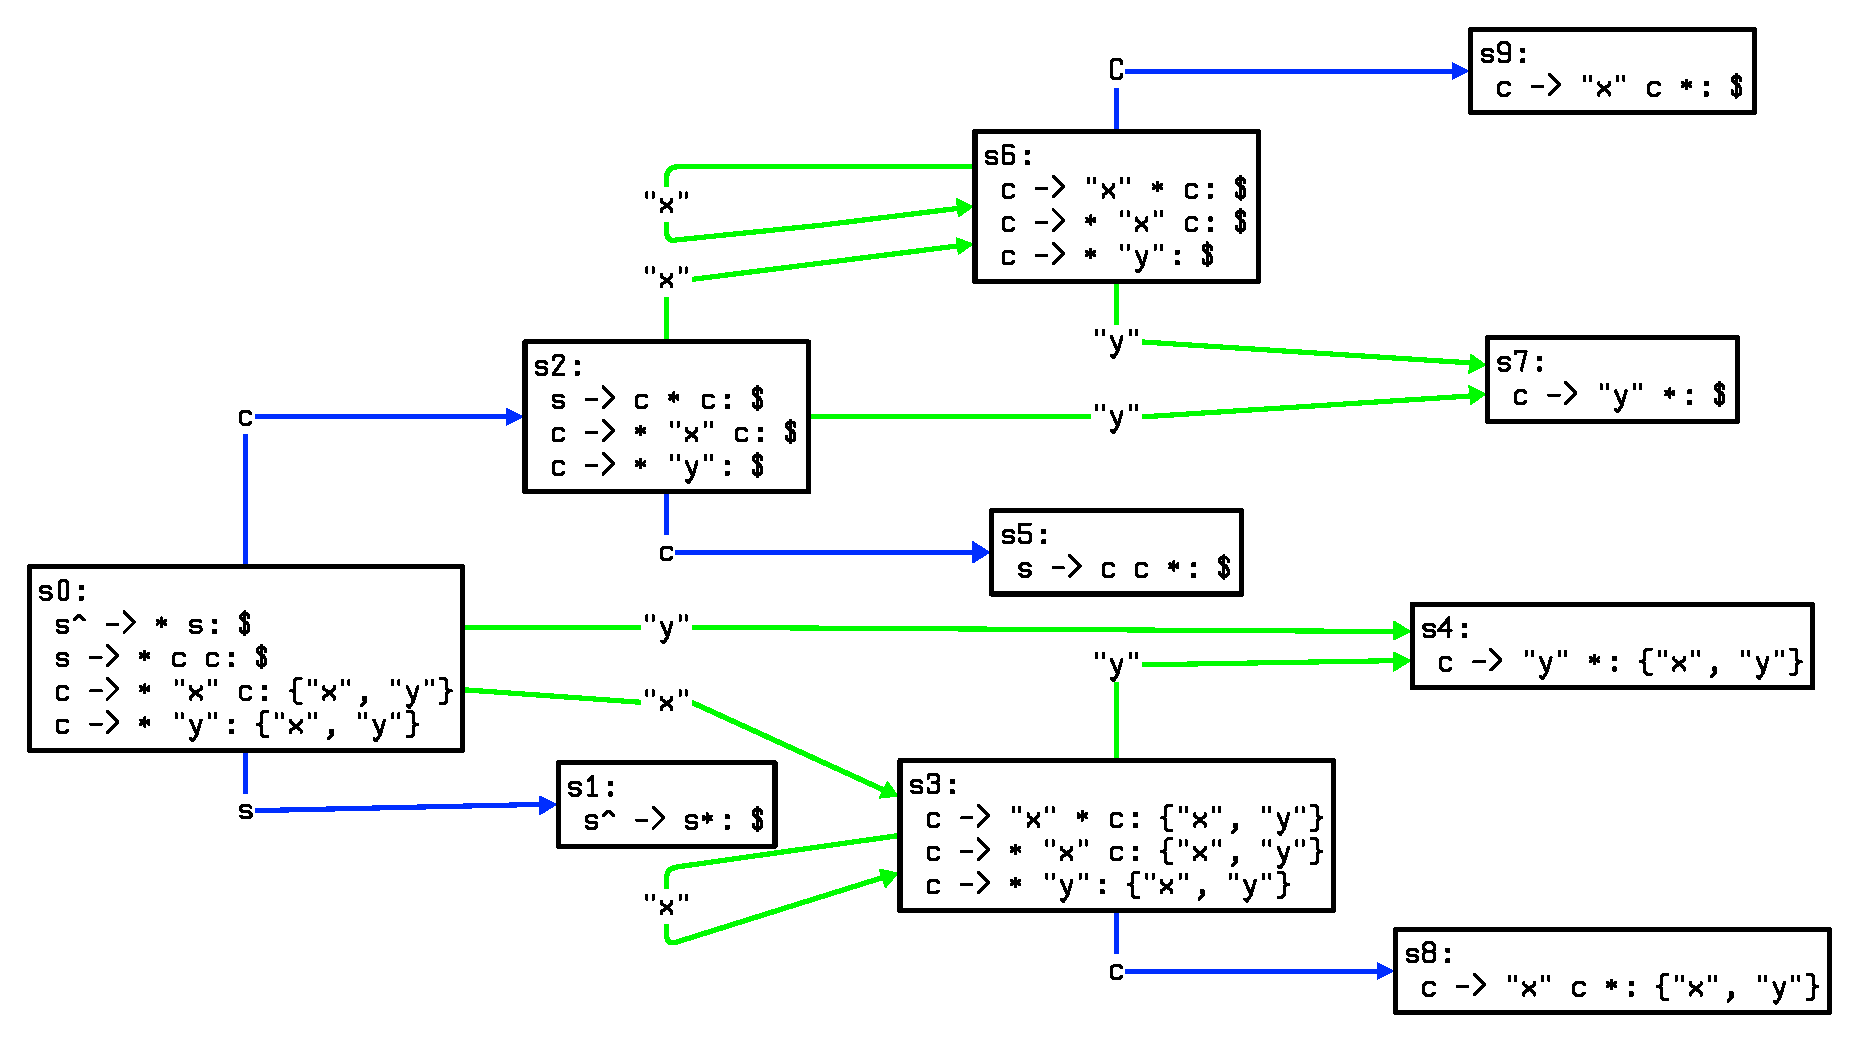
\epsfig{file=Abbildungen/cc-LR.eps, scale=0.5}
      \caption{LR-goto-graph for the grammar of Figure \ref{fig:dragon-book.grammar}.}
  \label{fig:cc-LR.eps}
\end{figure}

Figure \ref{fig:cc-LR.eps} shows the so-called \blue{LR-goto-graph} for this grammar.
The nodes of this graph are the states.  
Looking at the LR-goto-graph, we find that the states $s_6$ and
$s_3$ differ only in the sets of follow tokens, as on one hand, we have
\\[0.2cm]
\hspace*{1.3cm}
$s_6 = \Bigl\{ s \rightarrow \text{\saquoted{x}} \bullet c: \text{\saquoted{\symbol{36}}}, 
                 c \rightarrow \bullet\, \text{\aquoted{x}} c:  \text{\saquoted{\symbol{36}}},
                 c \rightarrow \bullet\, \text{\aquoted{y}}:    \text{\saquoted{\symbol{36}}}
       \Bigr\}$, 
\\[0.2cm]
and on the other hand, we have
\\[0.2cm]
\hspace*{1.3cm}
$s_3 = \Bigl\{ s \rightarrow \text{\saquoted{x}} \bullet c: \{ \text{\saquoted{x}}, \text{\saquoted{y}} \}, 
                 c \rightarrow \bullet\, \text{\aquoted{x}} c:  \{ \text{\saquoted{x}}, \text{\saquoted{y}} \},
                 c \rightarrow \bullet\, \text{\aquoted{y}}:    \{ \text{\saquoted{x}}, \text{\saquoted{y}} \}  
       \Bigr\}$.
\\[0.2cm]
Clearly, the set $s_3$ is derived from the set $s_6$ by replacing everywhere $\text{\saquoted{\symbol{36}}}$
with the set $\{ \text{\saquoted{x}}, \text{\saquoted{y}}\}$. Similarly, the set $s_7$ can be transformed into $s_4$,
and $s_9$ into $s_8$. The crucial realization is that the
function $\textsl{goto}()$ is invariant under this kind of transformation, because in the
definition of this function, the set of follow tokens is irrelevant. For example, we see that
\\[0.2cm]
\hspace*{1.3cm}
$\textsl{goto}(s_3, c) = s_8$ \quad and \quad 
$\textsl{goto}(s_6, c) = s_9$ 
\\[0.2cm]
hold and that, on the other hand, the state $s_9$ changes into the state $s_8$ when we
replace everywhere in $s_9$ the terminal $\text{\saquoted{\symbol{36}}}$ with the set 
 $\{ \text{\saquoted{x}}, \text{\saquoted{y}}\}$. If we define the \blue{core}
of a set of extended marked rules by omitting the set of follow tokens in each rule, and then combine states with the same core, we
obtain the goto-graph shown in Figure \ref{fig:cc-LALR.eps}.


\begin{figure}[!ht]
\centering
  \hspace*{-0.6cm} 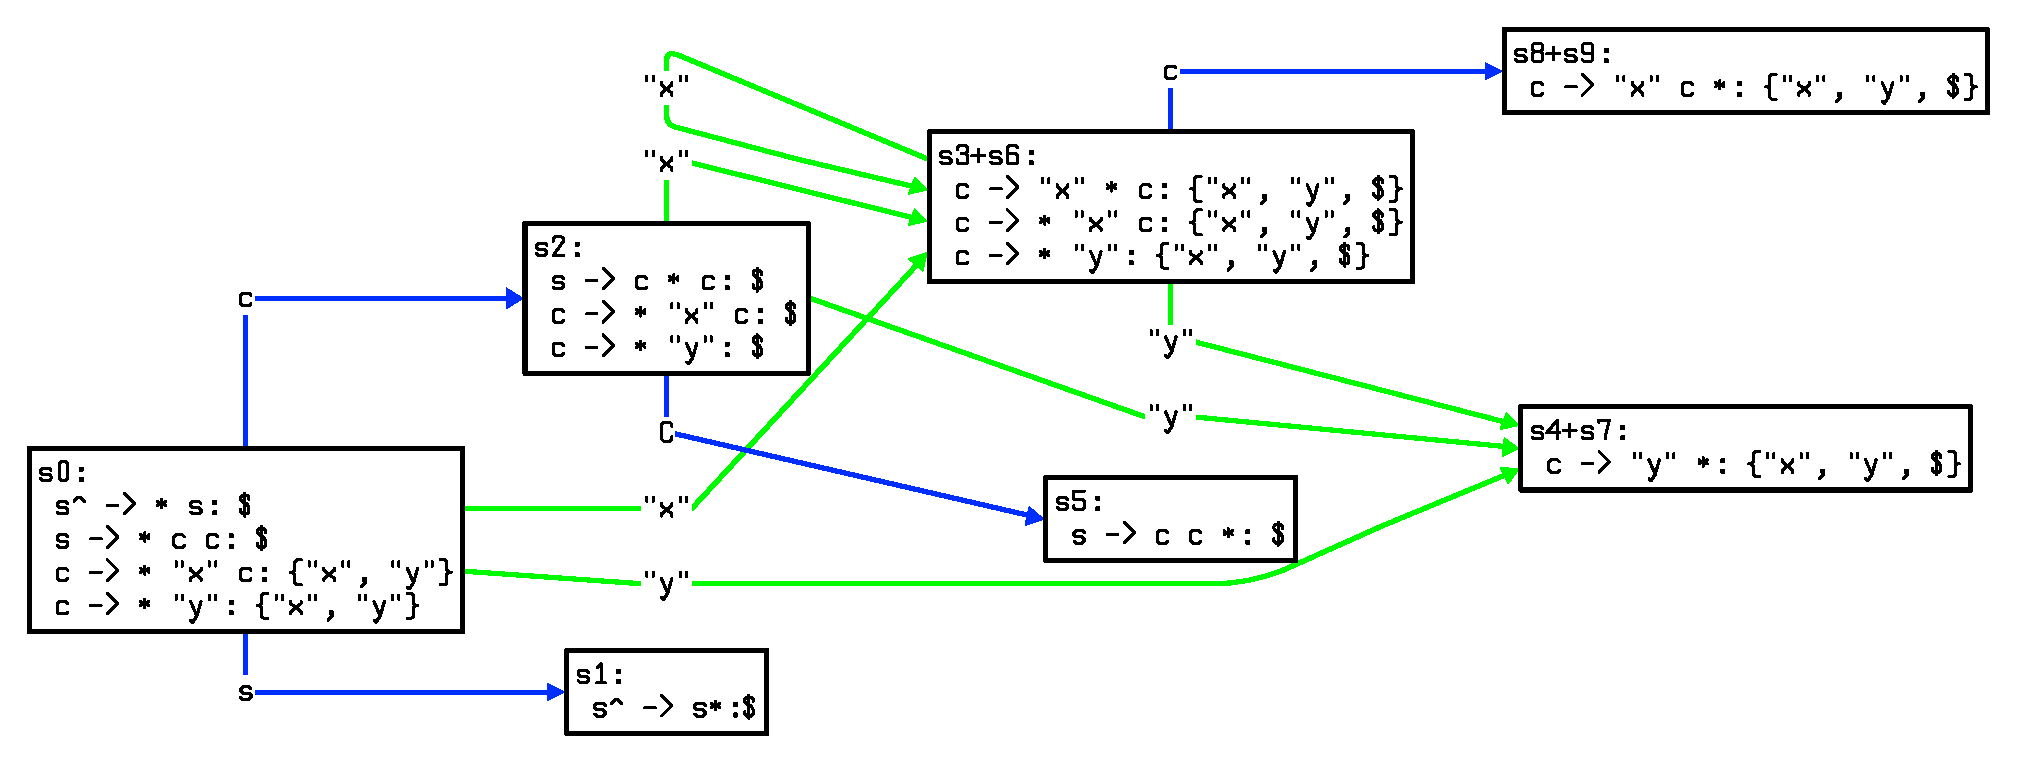
\epsfig{file=Abbildungen/cc-LALR, scale=0.5}
  \caption{The LALR-goto-graph for the grammar from Figure \ref{fig:dragon-book.grammar}.}
  \label{fig:cc-LALR.eps}
\end{figure}

To generalize and formalize the observations made while examining the grammar shown in Figure 
\ref{fig:dragon-book.grammar}, we define a function 
$\textsl{core}()$, which calculates the core of a set of e.m.R.s (extended marked rules) and thus transforms this set into 
a set of marked rules:
\\[0.2cm]
\hspace*{1.3cm}
$\textsl{core}(\mathcal{M}) := 
   \{ a \rightarrow \beta \bullet \gamma \mid (a \rightarrow \beta \bullet \gamma:L) \in \mathcal{M} \}$. 
\\[0.2cm]
Thus, the function $\textsl{core}()$ simply removes the set of follow tokens from the e.m.R.s.
We had defined the function $\textsl{goto}()$ for a set $\mathcal{M}$ of extended
marked rules and a symbol $x$ as
\\[0.2cm]
\hspace*{1.3cm}
$\textsl{goto}(\mathcal{M}, x) := \textsl{closure}\Bigl( \bigl\{ 
 a \rightarrow \beta\, x \bullet \gamma:L \mid (a \rightarrow \beta \bullet x\, \gamma:L) \in \mathcal{M} 
 \bigr\} \Bigr)
$.
\\[0.2cm]
Clearly, the set of follow tokens plays no role in the calculation of
$\textsl{goto}(\mathcal{M}, x)$, formally for two e.m.R.-sets
$\mathcal{M}_1$ and $\mathcal{M}_2$ and a symbol $x$, the formula holds:
\\[0.2cm]
\hspace*{1.3cm}
$\textsl{core}(\mathcal{M}_1) = \textsl{core}(\mathcal{M}_2) \;\Rightarrow\;
 \textsl{core}(\textsl{goto}(\mathcal{M}_1, x)) = 
 \textsl{core}(\textsl{goto}(\mathcal{M}_2, x))
$.
\vspace*{0.2cm}

For two sets of e.m.R.s (extended marked rules) $\mathcal{M}$ and $\mathcal{N}$ that
have the same core, we define the \blue{extended union}  
$\mathcal{M} \uplus \mathcal{N}$ of $\mathcal{M}$ and $\mathcal{N}$ as
\\[0.2cm]
\hspace*{1.3cm}
$\mathcal{M} \uplus \mathcal{N} := 
   \{ a \rightarrow \beta\bullet \gamma:K \cup L \mid 
      (a \rightarrow \beta\bullet \gamma:K) \in \mathcal{M} \;\wedge\;
      (a \rightarrow \beta\bullet \gamma:L) \in \mathcal{N}
   \}
$.
\\[0.2cm] 
We generalize this definition to an operation $\biguplus$, 
defined on a set of sets of e.m.R.s: If $\frak{I}$
is a set of sets of e.m.R.s, all having the same core, i.e.,
\[ \frak{I} = \{ \mathcal{M}_1, \cdots, \mathcal{M}_k \} \quad \mbox{with} \quad
   \textsl{core}(\mathcal{M}_i) = \textsl{core}(\mathcal{M}_j) \quad 
   \mbox{for all $i,j\in\{1,\cdots,k\}$,} 
\]
then we define
\[ \biguplus \frak{I} := \mathcal{M}_1 \uplus \cdots \uplus \mathcal{M}_k. 
\]
Let $\Delta$ be the set of all states of an LR parser. Then, the set of states of the
corresponding LALR parser is given by the extended union of all subsets 
of $\Delta$ whose elements have the same core:
\[ \frak{Q} := \left\{ \biguplus \frak{I} \mid \frak{I} \in 2^\Delta \wedge 
      \forall \mathcal{M},\mathcal{N} \in \frak{I}: \textsl{core}(\mathcal{M}) = \textsl{core}(\mathcal{N}) 
      \wedge \mbox{and $\frak{I}$ is maximal} 
   \right\}. 
\]
The requirement ``$\frak{I}$ maximal'' in the above definition expresses that in $\frak{I}$, indeed
\underline{all} sets from $\Delta$ are combined that have the same core.
The thus defined set $\frak{Q}$ is the set of LALR states.

Next, we consider how the computation of $\textsl{goto}(\mathcal{M},X)$
must change if $\mathcal{M}$ is an element of the set $\frak{Q}$ of LALR states.  
To compute $\textsl{goto}(\mathcal{M},X)$, we first calculate the set
\\[0.2cm]
\hspace*{1.3cm}
$\textsl{closure}\Bigl( \bigl\{  
  A \rightarrow \alpha X \bullet \beta:L \mid (A \rightarrow \alpha \bullet X \beta:L) \in \mathcal{M} 
  \bigr\} \Bigr)
$.
\\[0.2cm]
The problem is that this set is generally not an element of the set $\frak{Q}$,
as the states in $\frak{Q}$ arise from the combination of several LR states.
However, the states that are combined in the computation of $\frak{Q}$ all have the same
core. Therefore, the set
\\[0.2cm]
\hspace*{1.3cm}
$\Bigl\{ q \in \frak{Q} \mid \textsl{core}(q) =
  \textsl{core}\bigl(\textsl{closure}\bigl( \bigl\{  
  a \rightarrow \beta\, x \bullet \gamma:L \mid (a \rightarrow \beta \bullet x\, \gamma:L) \in \mathcal{M} 
  \bigr\} \bigr)\bigr)
  \Bigr\}
$
\\[0.2cm]
contains exactly one element and this element is the value of $\textsl{goto}(\mathcal{M}, X)$. Thus,
we can set
\\[0.2cm]
\hspace*{1.3cm}
$\ds\textsl{goto}(\mathcal{M}, X) := \textsl{arb}\Bigl(\Bigl\{ q \in \frak{Q} \mid \textsl{core}(q) =
  \textsl{core}\Bigl(\textsl{closure}\Bigl( \bigl\{  
  a \rightarrow \beta\, X \bullet \gamma:L \mid (a \rightarrow \beta \bullet X\, \gamma:L) \in \mathcal{M} 
  \bigr\} \Bigr)\Bigr)
  \Bigr\} \Bigr)
$
\\[0.2cm]
The function $\textsl{arb}()$ used here serves to extract an arbitrary element from a set.
Since the set from which the element is extracted contains exactly one element, 
$\textsl{goto}(\mathcal{M}, x)$ is well-defined.
The computation of the expression $\textsl{action}(\mathcal{M}, t)$ does not change compared to the computation for
an LR parser.

\section{Comparison of SLR, LR, and LALR Parsers}
We now want to compare the different methods with which we have constructed Shift-Reduce parsers in this
chapter. We call a language $\mathcal{L}$ 
an \blue{SLR language} if $\mathcal{L}$ can be recognized by an SLR parser.
The terms \blue{canonical LR language} and \blue{LALR language} are defined analogously.
The following relationships exist between these languages:
\\[0.2cm]
\hspace*{1.3cm}
\blue{SLR language} $\subsetneq$ \blue{LALR language} $\subsetneq$ \blue{canonical LR language} 
\hspace*{\fill} $(\star)$
\\[0.2cm]
These inclusions are easy to understand: In defining the LR parsers, we
added sets of follow tokens to the marked rules. This made it
possible to avoid Shift-Reduce and Reduce-Reduce conflicts in certain cases.
As the state sets of canonical LR parsers can become very large,
we then combined sets of extended marked rules that have the same core. This is how we
obtained the LALR parsers. However, by combining rule sets, we can
in some cases introduce Reduce-Reduce conflicts, so the 
set of LALR languages is a subset of the canonical LR languages.

We will show in the following subsections that the inclusions in $(\star)$ are proper.

\subsection{\blue{SLR Language} $\subsetneq$ \blue{LALR Language}}
The states of an LALR parser, as compared to those of an SLR parser, include sets of follow tokens. This makes LALR parsers at least as powerful as SLR parsers. We will now demonstrate that LALR parsers are indeed more powerful than SLR parsers. To support this claim, we present a grammar for which there exists an LALR parser, but no SLR parser. We had seen on page \pageref{fig:reduce-reduce-conflict.grammar} that the grammar
\\[0.2cm]
\hspace*{1.3cm}
$s \;\rightarrow\; a \text{\aquoted{x}} a \text{\aquoted{y}} \mid b \text{\aquoted{y}} b \text{\aquoted{x}}$
\\
\hspace*{1.3cm}
$a \;\rightarrow\;\lambda$ \quad
\\
\hspace*{1.3cm}
$b \;\rightarrow\; \lambda$
\\[0.2cm]
is not an SLR grammar. Later, we saw that this grammar can be parsed by a
canonical LR parser. We will now show that this grammar can also be parsed by
an LALR parser. To do this, we calculate the set of LALR states.
This requires first calculating the set of canonical LR states. We had already carried out this calculation earlier and obtained the following states:
\begin{enumerate}
\item $s_0  = \bigl\{ \widehat{s} \rightarrow \bullet\, s:\symbol{36},
                     s \rightarrow \bullet\, a \saquoted{x} a \saquoted{y}:\symbol{36},
                     s \rightarrow \bullet\, b \saquoted{y} b \saquoted{x}:\symbol{36},
                     a \rightarrow \bullet\,: \saquoted{x},
                     b \rightarrow \bullet\,: \saquoted{y}
              \bigr\}
      $,
\item $s_1 = \bigl\{ s \rightarrow a \bullet \saquoted{x} a \saquoted{y}:\symbol{36} \bigr\}$,
\item $s_2 = \bigl\{ \widehat{s} \rightarrow s \bullet:\symbol{36} \bigr\}$,
\item $s_3 = \bigl\{ s \rightarrow b \bullet \saquoted{y} b \saquoted{x}: \symbol{36} \bigr\}$,
\item $s_4 = \bigl\{ s \rightarrow b \saquoted{y} \bullet b \saquoted{x}: \symbol{36},
                     b \rightarrow \bullet\,: \saquoted{x}
             \bigr\}
      $,
\item $s_5 = \bigl\{ s \rightarrow b \saquoted{y} b \bullet \saquoted{x}: \symbol{36} \bigr\}$,
\item $s_6 = \bigl\{ s \rightarrow b \saquoted{y} b \saquoted{x} \bullet: \symbol{36} \bigr\}$,
\item $s_7 = \bigl\{ s \rightarrow a \saquoted{x} \bullet a \saquoted{y}:\symbol{36},
                     a \rightarrow \bullet\,: \saquoted{y}
              \bigr\}
      $,
\item $s_8 = \bigl\{ s \rightarrow a \saquoted{x} a \bullet \saquoted{y}:\symbol{36} \bigr\}$,
\item $s_9 = \bigl\{ s \rightarrow a \saquoted{x} a \saquoted{y} \bullet :\symbol{36} \bigr\}$.
\end{enumerate}
We observe that the cores of all the states listed here are different.
Therefore, for this grammar, the set of states of the LALR parser coincides with the set of
states of the canonical LR parser. This implies that there are no conflicts in the
LALR states, because in the transition from canonical LR parsers to
LALR parsers, we have only combined states with the same core, and the
definition of the functions $\textsl{goto}()$ and $\textsl{action}()$ remained unchanged.
 
\subsection{\blue{LALR Language} $\subsetneq$ \blue{Canonical LR Language}}
We defined LALR parsers by combining different states of a canonical LR parser. Therefore, it is clear that canonical LR parsers are at least as powerful as LALR parsers. To demonstrate that canonical LR parsers are indeed more powerful than LALR parsers, we need a grammar for which a canonical LR parser can be generated, but not an LALR parser. Figure \ref{fig:lr-but-notlalr.g} shows such a grammar, which I have taken from the Dragon Book.

\begin{figure}[htbp]
  \begin{center}    
  \framebox{
  \framebox{
  \begin{minipage}[t]{5.5cm}
    \vspace*{-0.3cm}

  \begin{eqnarray*}
  s  & \rightarrow & \aquoted{v} a \aquoted{y} \\
     & \mid        & \aquoted{w} b \aquoted{y} \\
     & \mid        & \aquoted{v} b \aquoted{z} \\
     & \mid        & \aquoted{w} a \aquoted{z} \\[0.1cm]
  a  & \rightarrow & \aquoted{x}              \\[0.1cm]
  b  & \rightarrow & \aquoted{x}              
  \end{eqnarray*}
  \vspace*{-0.5cm}

  \end{minipage}}}
  \vspace*{-0.3cm}

  \end{center}
  \caption{A canonical LR grammar that is not an LALR grammar.}
  \label{fig:lr-but-notlalr.g}
\end{figure}

We first calculate the set of states for a canonical LR parser for this grammar. We obtain the following sets
of extended marked rules: 
\begin{enumerate}
\item $s_0 = \textsl{closure}(\widehat{s} \rightarrow \bullet\, \;s: \symbol{36}) =
       \{
       \begin{array}[t]{lcl}
         \widehat{s} & \rightarrow & \bullet \;s: \symbol{36},                \\
         s           & \rightarrow & \bullet \saquoted{v} a \saquoted{y}: \symbol{36}, \\
         s           & \rightarrow & \bullet \saquoted{v} b \saquoted{z}: \symbol{36}, \\
         s           & \rightarrow & \bullet \saquoted{w} a \saquoted{z}: \symbol{36}, \\
         s           & \rightarrow & \bullet \saquoted{w} b \saquoted{y}: \symbol{36}\;\},
        \end{array}
       $
\item $s_1 = \textsl{goto}(s_0, s) =\{ \widehat{s} \rightarrow s \bullet: \symbol{36} \}$
\item $s_2 = \textsl{goto}(s_0, \aquoted{v}) = \{ 
       \begin{array}[t]{lcl}
        s & \rightarrow & \saquoted{v} \bullet b \saquoted{z}: \symbol{36}, \\
        s & \rightarrow & \saquoted{v} \bullet a \saquoted{y}: \symbol{36}, \\
        a & \rightarrow & \bullet \saquoted{x}: \saquoted{y}, \\
        b & \rightarrow & \bullet \saquoted{x}: \saquoted{z}\; \},
       \end{array}
      $
\item $s_3 = \textsl{goto}(s_0, \aquoted{w}) = \{ 
       \begin{array}[t]{lcl}
       s & \rightarrow & \saquoted{w} \bullet a \saquoted{z}: \symbol{36},  \\
       s & \rightarrow & \saquoted{w} \bullet b \saquoted{y}: \symbol{36},  \\
       a & \rightarrow & \bullet \saquoted{x}: \saquoted{z},                \\
       b & \rightarrow & \bullet \saquoted{x}: \saquoted{y}\; \},
       \end{array}
      $
\item $s_4 = \textsl{goto}(s_2, \aquoted{x}) =
             \{ a \rightarrow \saquoted{x} \bullet: \saquoted{y},\;
                b \rightarrow \saquoted{x} \bullet: \saquoted{z} \}$,
\item $s_5 = \textsl{goto}(s_3, \aquoted{x}) =
             \{ a \rightarrow \saquoted{x} \bullet: \saquoted{z},\,
                b \rightarrow \saquoted{x} \bullet: \saquoted{y} \}$,
\item $s_6 = \textsl{goto}(s_2, a) =
             \{ s \rightarrow \saquoted{v} a \bullet \saquoted{y}: \symbol{36} \}$,
\item $s_7 = \textsl{goto}(s_6, \aquoted{y}) =
             \{ s \rightarrow \saquoted{v} a \saquoted{y} \bullet: \symbol{36} \}$,
\item $s_8 = \textsl{goto}(s_2, b) =
             \{ s \rightarrow \saquoted{v} b \bullet \saquoted{z}: \symbol{36} \}$,
\item $s_9 = \textsl{goto}(s_8, \aquoted{z}) =
             \{ s \rightarrow \saquoted{v} b \saquoted{z} \bullet: \symbol{36} \}$,
\item $s_{10} = \textsl{goto}(s_3, a) =
                \{ s \rightarrow \saquoted{w} a \bullet \saquoted{z}: \symbol{36} \}$,
\item $s_{11} = \textsl{goto}(s_{10}, \aquoted{z}) =
                \{ s \rightarrow \saquoted{w} a \saquoted{z} \bullet: \symbol{36} \}$,
\item $s_{12} = \textsl{goto}(s_3, b) =
                \{ s \rightarrow \saquoted{w} b \bullet \saquoted{y}: \symbol{36} \}$,
\item $s_{13} = \textsl{goto}(s_{12}, \aquoted{y}) =
                \{ s \rightarrow \saquoted{w} b \saquoted{y} \bullet: \symbol{36} \}$.
\end{enumerate}
The only states where conflicts could occur are the sets $s_4$ and $s_5$, as in these states, reductions with both rules
\\[0.2cm]
\hspace*{1.3cm}
$a \rightarrow \saquoted{x}$ \quad and \quad
$b \rightarrow \saquoted{x}$
\\[0.2cm]
are potentially possible. However, since the sets of follow tokens have an empty intersection, there is actually no conflict, and the grammar is a canonical LR grammar.

Next, we calculate the LALR states for the grammar mentioned above. The only states that have a common core are $s_4$ and $s_5$, as
\\[0.2cm]
\hspace*{1.3cm}
$\textsl{core}(s_4) = \{ a \rightarrow \saquoted{x} \bullet,\;
                b \rightarrow \saquoted{x} \bullet \} = \textsl{core}(s_5)$.
\\[0.2cm]
In calculating the LALR states, these two states are combined into one state $s_{\{4,5\}}$. This new state takes the form
\\[0.2cm]
\hspace*{1.3cm}
$s_{\{4,5\}} = \bigl\{ A \rightarrow \saquoted{x} \bullet: \{\saquoted{y}, \saquoted{z} \},\;
                       B \rightarrow \saquoted{x} \bullet: \{\saquoted{y}, \saquoted{z} \} \bigr\}$.
\\[0.2cm]
Here, there is obviously a reduce-reduce conflict, as on one hand we have
\\[0.2cm]
\hspace*{1.3cm}
$\textsl{action}(s_{\{4,5\}}, \saquoted{y}) = \pair(\textsl{reduce}, A \rightarrow \saquoted{x})$,
\\[0.2cm]
but on the other hand, it also holds that
\\[0.2cm]
\hspace*{1.3cm}
$\textsl{action}(s_{\{4,5\}}, \saquoted{y}) = \pair(\textsl{reduce}, B \rightarrow \saquoted{x})$.

\exerciseEng
Let $G = \langle V, T, R, s \rangle$ be an LR grammar and $\mathcal{N}$ be the set of LALR states of the grammar. Explain why there can be no shift-reduce conflicts in the set $\mathcal{N}$. \eox

\paragraph{Historical Notes}
The theory of LALR parsing is due to Franklin L.~DeRemer \cite{deRemer:71}.  At the time of its
invention,  the space savings of LALR parsing in comparison to LR parsing were crucial.  

\subsection{Evaluation of the Different Methods}
In practice, SLR parsers are not sufficient, as there are a number of practically relevant language constructs for which no SLR parser can be generated. Canonical LR parsers are much more powerful but often require significantly more states. LALR parsers represent a compromise here: on the one hand, LALR languages are almost as expressive as canonical LR languages, but on the other hand, the memory requirements of LALR parsers are in the same order of magnitude as those of SLR parsers. For example, the SLR parse table for the \texttt{C} language has a total of 349 states, the corresponding LR parse table has 1572 states, while the LALR parser manages with 350 states, thus only one state more than the SLR parser.  
In the main memories typically available today, however, canonical LR parsers can usually be accommodated without difficulty, so there is actually no compelling reason to use an LALR parser instead of an LR parser.  

On the other hand, no one will want to program an LALR parser or a canonical LR parser by hand. Instead, you will later use a parser generator like \textsl{Bison} or \textsl{JavaCup}, which generates a parser for you. Bison is a parser generator for \texttt{C}, \texttt{C++} and also offers, albeit still experimental, support for \textsl{Java}, while \textsl{JavaCup} is limited to the language \textsl{Java}. If you use \textsl{JavaCup}, you have no choice, as this tool always generates an LALR parser. With \href{http://www.gnu.org/software/bison/manual/bison.html}{\textsl{Bison}}, from version 3.0, it is also possible to generate an LR parser.

\section{Check your Understanding}
\begin{enumerate}[(a)]
\item What is the definition of a \blue{shift-reduce parser} and how is the set \textsl{Action} defined?
\item How does a shift-reduce parser work?

      If you are unsure about this question, you should run the notebook
      \\[0.2cm]
      \hspace*{-0.6cm}
      \href{https://github.com/karlstroetmann/Formal-Languages/blob/master/Python/Chapter-09/Shift-Reduce-Parser.ipynb}{https://github.com/karlstroetmann/Formal-Languages/blob/master/Python/Chapter-09/Shift-Reduce-Parser.ipynb}
      \\[0.2cm]
      and inspect its output.
\item How is the concept of a \blue{marked rule} defined?  How is a marked rule interpreted?
\item Can you compute the closure of a set of marked rules?
\item Are you able to define the functions \texttt{First} and \texttt{Follow} for an \textsc{Slr}-parser?
\item Are you able to compute the states of an \textsc{Slr}-parser?
\item Given the set of all states of an \textsc{Slr}-parser, can you compute both the action table and the goto
      table? 
\item How is the concept of an \blue{extended marked rule} defined?
\item Can you compute the closure of a set of extended marked rules?
\item Why are \textsc{Lr}-parser-generators more powerful than \textsc{Slr}-parser-generators?
\end{enumerate}


%%% Local Variables: 
%%% mode: latex
%%% TeX-master: "formal-languages"
%%% End: 
